\documentclass[twocolumn,traditabstract]{aa}
%\documentclass[referee]{aa}
\usepackage{fixltx2e}
\usepackage[english]{babel}
\usepackage{graphicx,amsmath}
%\usepackage{epstopdf}
\usepackage{epsf,color}
\usepackage[mathscr]{eucal}
\usepackage{amsmath}
\usepackage{amssymb,amsfonts}
\usepackage{natbib}
\usepackage{txfonts}
\usepackage{dsfont}
\definecolor{Mygreen}{rgb}{0.00, 0.72, 0.0}
\definecolor{Mypink}{rgb}{1.0, 0.0, 0.5}
\usepackage[breaklinks, citecolor=blue, linkcolor=Mygreen, urlcolor=Mypink, colorlinks=true, debug, baseurl=' ']{hyperref}
\usepackage{float}
\usepackage{color}
%\usepackage{scrextend}
%\usepackage{nccmath}
%\usepackage{mathtools, cuted}
%\usepackage{lscape}
%\usepackage{widetext}
%\usepackage{flushend}
%\usepackage[T1]{fontenc}


\newcommand{\nika}{{\it NIKA}}
\newcommand{\nikad}{{\it NIKA2}}


\def\intk#1{\displaystyle\int\frac{d^2k_{#1}}{(2\pi)^2}}
\def\intr#1{\displaystyle\int d^2r_{#1}}
\def\simlt{\lower.5ex\hbox{$\; \buildrel < \over \sim \;$}}
\def\simgt{\lower.5ex\hbox{$\; \buildrel > \over \sim \;$}}
\def\simgt{\lower.5ex\hbox{$\; \buildrel $\textgreater$ \over \sim \;$}}
\def\NIKA{\textit{NIKA}}
\def\NIKAd{\textit{NIKA2}}
\def\Archeops{\textit{Archeops}}
\def\Planck{\textit{Planck}}
\def\WMAP{\textit{WMAP}}
\def\Skydip{\textit{Skydip}}

\bibpunct{(}{)}{;}{a}{}{,}
\bibliographystyle{aa}

\begin{document}
\title{Crab nebula polarization observations at 150 GHz with NIKA}
\author{A.~Ritacco \inst{\ref{LPSC}},\inst{\ref{IRAME}}\thanks{Corresponding author: Alessia Ritacco, \url{ritaccoa@iram.es}}
\and  J.F.~Mac\'ias-P\'erez \inst{\ref{LPSC}}
\and  N.~Ponthieu \inst{\ref{IPAG}}
\and  R.~Adam \inst{\ref{LPSC},\ref{OCA}}
\and  P.~Ade \inst{\ref{Cardiff}}
\and  P.~Andr\'e \inst{\ref{CEA}}
\and  A.~Beelen \inst{\ref{IAS}}
\and  A.~Beno\^it \inst{\ref{Neel}}
\and  A.~Bideaud \inst{\ref{Neel}}
\and  N.~Billot \inst{\ref{IRAME}}
\and  O.~Bourrion \inst{\ref{LPSC}}
\and  A.~Bracco \inst{\ref{CEA}}
\and  M.~Calvo \inst{\ref{Neel}}
\and  A.~Catalano \inst{\ref{LPSC}}
\and  G.~Coiffard \inst{\ref{IRAMF}}
\and  B.~Comis \inst{\ref{LPSC}}
\and  A.~D'Addabbo \inst{\ref{Neel},\ref{Roma}}
\and  F.-X.~D\'esert \inst{\ref{IPAG}}
\and  S.~Doyle \inst{\ref{Cardiff}}
\and  J.~Goupy \inst{\ref{Neel}}
\and  C.~Kramer \inst{\ref{IRAME}}
\and  G.~Lagache \inst{\ref{LAM}}
\and  S.~Leclercq \inst{\ref{IRAMF}}
\and  J.-F.~Lestrade \inst{\ref{LERMA}}
\and  P.~Mauskopf \inst{\ref{Cardiff},\ref{Arizona}}
\and  F.~Mayet \inst{\ref{LPSC}}
\and  A.~Maury \inst{\ref{CEA}}
\and  A.~Monfardini \inst{\ref{Neel}}
\and  F.~Pajot \inst{\ref{IAS}}
\and  E.~Pascale \inst{\ref{Cardiff}}
\and  L.~Perotto \inst{\ref{LPSC}}
\and  G.~Pisano \inst{\ref{Cardiff}}
\and  M.~Rebolo-Iglesias\inst{\ref{LPSC}}
\and  V.~Rev\'eret \inst{\ref{CEA}}
\and  L.~Rodriguez \inst{\ref{CEA}}
\and  C.~Romero \inst{\ref{IRAMF}}
\and  H.~Roussel \inst{\ref{IAP}}
\and  F.~Ruppin \inst{\ref{LPSC}}
\and  K.~Schuster \inst{\ref{IRAMF}}
\and  A.~Sievers \inst{\ref{IRAME}}
\and  C.~Thum \inst{\ref{IRAME}}
\and  S.~Triqueneaux \inst{\ref{Neel}}
\and  C.~Tucker \inst{\ref{Cardiff}}
\and  R.~Zylka \inst{\ref{IRAMF}}}

\institute{
Laboratoire de Physique Subatomique et de Cosmologie, Universit\'e Grenoble Alpes, CNRS/IN2P3, 53, avenue des Martyrs, Grenoble, France
  \label{LPSC}
  \and
  Laboratoire Lagrange, Universit\'e C\^ote d'Azur, Observatoire de la C\^ote d'Azur, CNRS, Blvd de l'Observatoire, CS 34229, 06304 Nice cedex 4, France
  \label{OCA}
  \and
Institut de RadioAstronomie Millim\'etrique (IRAM), Grenoble, France
  \label{IRAMF}
\and
Laboratoire AIM, CEA/IRFU, CNRS/INSU, Universit\'e Paris Diderot, CEA-Saclay, 91191 Gif-Sur-Yvette, France 
  \label{CEA}
\and
Astronomy Instrumentation Group, University of Cardiff, UK
  \label{Cardiff}
\and
Institut d'Astrophysique Spatiale (IAS), CNRS and Universit\'e Paris Sud, Orsay, France
  \label{IAS}
\and
Institut N\'eel, CNRS and Universit\'e Grenoble Alpes, France
  \label{Neel}
\and
Institut de RadioAstronomie Millim\'etrique (IRAM), Granada, Spain
  \label{IRAME}
\and
Dipartimento di Fisica, Sapienza Universit\`a di Roma, Piazzale Aldo Moro 5, I-00185 Roma, Italy
  \label{Roma}
\and
Univ. Grenoble Alpes, CNRS, IPAG, F-38000 Grenoble, France 
  \label{IPAG}
    \and
Aix Marseille Universit\'e, CNRS, LAM (Laboratoire d'Astrophysique de Marseille) UMR 7326, 13388, Marseille, France
  \label{LAM}
\and
School of Earth and Space Exploration and Department of Physics, Arizona State University, Tempe, AZ 85287
  \label{Arizona}
\and
Universit\'e de Toulouse, UPS-OMP, Institut de Recherche en Astrophysique et Plan\'etologie (IRAP), Toulouse, France
  \label{IRAP}
\and
CNRS, IRAP, 9 Av. colonel Roche, BP 44346, F-31028 Toulouse cedex 4, France 
  \label{IRAP2}
\and
University College London, Department of Physics and Astronomy, Gower Street, London WC1E 6BT, UK
  \label{UCL}
\and  
Institut d'Astrophysique de Paris, Sorbonne Universit\'es,
  UPMC Univ. Paris 06, CNRS UMR 7095, 75014 Paris, France
\label{IAP}
\and
LERMA, CNRS, Observatoire de Paris, 61 avenue de l'Observatoire, Paris, France
  \label{LERMA}}
%\author{A.~Ritacco \inst{\ref{LPSC}}\thanks{Corresponding author: Alessia Ritacco, \url{ritacco@lpsc.in2p3.fr}}
\and  N.~Ponthieu \inst{\ref{IPAG}}
\and  A.~Catalano \inst{\ref{LPSC}}
\and R.~Adam \inst{\ref{LPSC},\ref{OCA}}
\and  P.~Ade \inst{\ref{Cardiff}}
\and  P.~Andr\'e \inst{\ref{CEA}}
\and  A.~Beelen \inst{\ref{IAS}}
\and  A.~Beno\^it \inst{\ref{Neel}}
\and  A.~Bideaud \inst{\ref{Neel}}
\and  N.~Billot \inst{\ref{IRAME}}
\and  O.~Bourrion \inst{\ref{LPSC}}
\and  M.~Calvo \inst{\ref{Neel}}
\and  G.~Coiffard \inst{\ref{IRAMF}}
\and  B.~Comis \inst{\ref{LPSC}}
\and  F.-X.~D\'esert \inst{\ref{IPAG}}
\and  S.~Doyle \inst{\ref{Cardiff}}
\and  J.~Goupy \inst{\ref{Neel}}
\and  C.~Kramer \inst{\ref{IRAME}}
\and  S.~Leclercq \inst{\ref{IRAMF}}
\and  J.F.~Mac\'ias-P\'erez \inst{\ref{LPSC}}
\and  P.~Mauskopf \inst{\ref{Cardiff},\ref{Arizona}}
\and A. Maury \inst{\ref{CEA}}
\and  F.~Mayet \inst{\ref{LPSC}}
\and  A.~Monfardini \inst{\ref{Neel}}
\and  F.~Pajot \inst{\ref{IAS}}
\and  E.~Pascale \inst{\ref{Cardiff}}
\and  L.~Perotto \inst{\ref{LPSC}}
\and  G.~Pisano \inst{\ref{Cardiff}}
\and M.~Rebolo-Iglesias  \inst{\ref{LPSC}}
\and  V.~Rev\'eret \inst{\ref{CEA}}
\and  L.~Rodriguez \inst{\ref{CEA}}
\and  C.~Romero \inst{\ref{IRAMF}}
\and F.~Ruppin \inst{\ref{LPSC}}
\and G.~Savini \inst{\ref{London_college}}
\and  K.~Schuster \inst{\ref{IRAMF}}
\and  A.~Sievers \inst{\ref{IRAME}}
\and C. Thum \inst{\ref{IRAME}}
\and  S.~Triqueneaux \inst{\ref{Neel}}
\and  C.~Tucker \inst{\ref{Cardiff}}
\and  R.~Zylka \inst{\ref{IRAMF}}}

%\institute{
Laboratoire de Physique Subatomique et de Cosmologie, Universit\'e Grenoble Alpes, CNRS/IN2P3, 53, avenue des Martyrs, Grenoble, France
  \label{LPSC}
  \and
  Laboratoire Lagrange, Universit\'e C\^ote d'Azur, Observatoire de la C\^ote d'Azur, CNRS, Blvd de l'Observatoire, CS 34229, 06304 Nice cedex 4, France
  \label{OCA}
  \and
Institut de RadioAstronomie Millim\'etrique (IRAM), Grenoble, France
  \label{IRAMF}
\and
Laboratoire AIM, CEA/IRFU, CNRS/INSU, Universit\'e Paris Diderot, CEA-Saclay, 91191 Gif-Sur-Yvette, France 
  \label{CEA}
\and
Astronomy Instrumentation Group, University of Cardiff, UK
  \label{Cardiff}
\and
Institut d'Astrophysique Spatiale (IAS), CNRS and Universit\'e Paris Sud, Orsay, France
  \label{IAS}
\and
Institut N\'eel, CNRS and Universit\'e Grenoble Alpes, France
  \label{Neel}
\and
Institut de RadioAstronomie Millim\'etrique (IRAM), Granada, Spain
  \label{IRAME}
\and
Dipartimento di Fisica, Sapienza Universit\`a di Roma, Piazzale Aldo Moro 5, I-00185 Roma, Italy
  \label{Roma}
\and
Univ. Grenoble Alpes, CNRS, IPAG, F-38000 Grenoble, France 
  \label{IPAG}
    \and
Aix Marseille Universit\'e, CNRS, LAM (Laboratoire d'Astrophysique de Marseille) UMR 7326, 13388, Marseille, France
  \label{LAM}
\and
School of Earth and Space Exploration and Department of Physics, Arizona State University, Tempe, AZ 85287
  \label{Arizona}
\and
Universit\'e de Toulouse, UPS-OMP, Institut de Recherche en Astrophysique et Plan\'etologie (IRAP), Toulouse, France
  \label{IRAP}
\and
CNRS, IRAP, 9 Av. colonel Roche, BP 44346, F-31028 Toulouse cedex 4, France 
  \label{IRAP2}
\and
University College London, Department of Physics and Astronomy, Gower Street, London WC1E 6BT, UK
  \label{UCL}
\and 
Institut d'Astrophysique de Paris, CNRS (UMR7095), 98 bis boulevard Arago, F-75014, Paris, France
  \label{IAP}
\and 
LERMA, CNRS, Observatoire de Paris, 61 avenue de l'Observatoire, Paris, France
  \label{LERMA}
}

\date{Received \today \ / Accepted --}
	
\abstract{The detection of the primordial Cosmic Microwave Background (CMB) polarization B-modes constitutes
  one of the major challenges of modern cosmology. Their precise measurement
  requires an accurate determination of foreground contaminants as well as of the
  absolute calibration of the instrument in terms of cross polarization and
  absolute polarization angle reconstruction. We present here a study of the
  Crab nebula, a supernova remnant, which is a well known calibration source in temperature and commonly used in polarization. The
  Crab nebula is the brightest source in the microwave sky with an extension
  of a few arcminutes corresponding to the typical beam-width of current CMB
  experiments. The Crab nebula exhibits highly polarized synchrotron radiation
  at radio and millimeter wavelengths. In addition to CMB measurements, it can be used as standard calibrator for any experiment 
  which aims at measuring the polarization of the sky. We report in this paper high resolution
  (18$^{\prime\prime}$ FWHM) observations of the Crab nebula in total intensity and
  linear polarization at 150 GHz with the \NIKA\ camera.  \NIKA, operated at the IRAM
  30 m telescope from 2012 to 2015, is a camera made of Lumped Element Kinetic
  Inductance Detectors (LEKIDs) observing the sky at 150 and 260 GHz.  From
  these observations we are able to reconstruct the spatial distribution of the
  Crab nebula polarization degree and angle, which is found to be compatible
  with previous observations at lower and higher frequencies.  Averaging across
  the source and using other existing data sets we find that the Crab nebula
  polarization angle is consistent with being constant over a wide range of frequencies with a
  value of $ -88.1^{\circ} \pm 0.3$ in Galactic coordinates.  We also present the first estimation of the Crab nebula Spectral Energy Distribution polarized flux.  These measurements will
  be crucial to calibrate current and next generation of CMB experiments operating at
  microwave wavelengths. } \titlerunning{NIKA polarisation observations of the
  Crab nebula.}  \authorrunning{A. Ritacco, J. F. Mac\'ias P\'erez , N. Ponthieu
  et al.}  \keywords{Techniques: Crab nebula -- Tau A -- polarization -- KIDs -- individual: NIKA }
\maketitle
\begin{figure*}[h!]
  \centering
     	  { 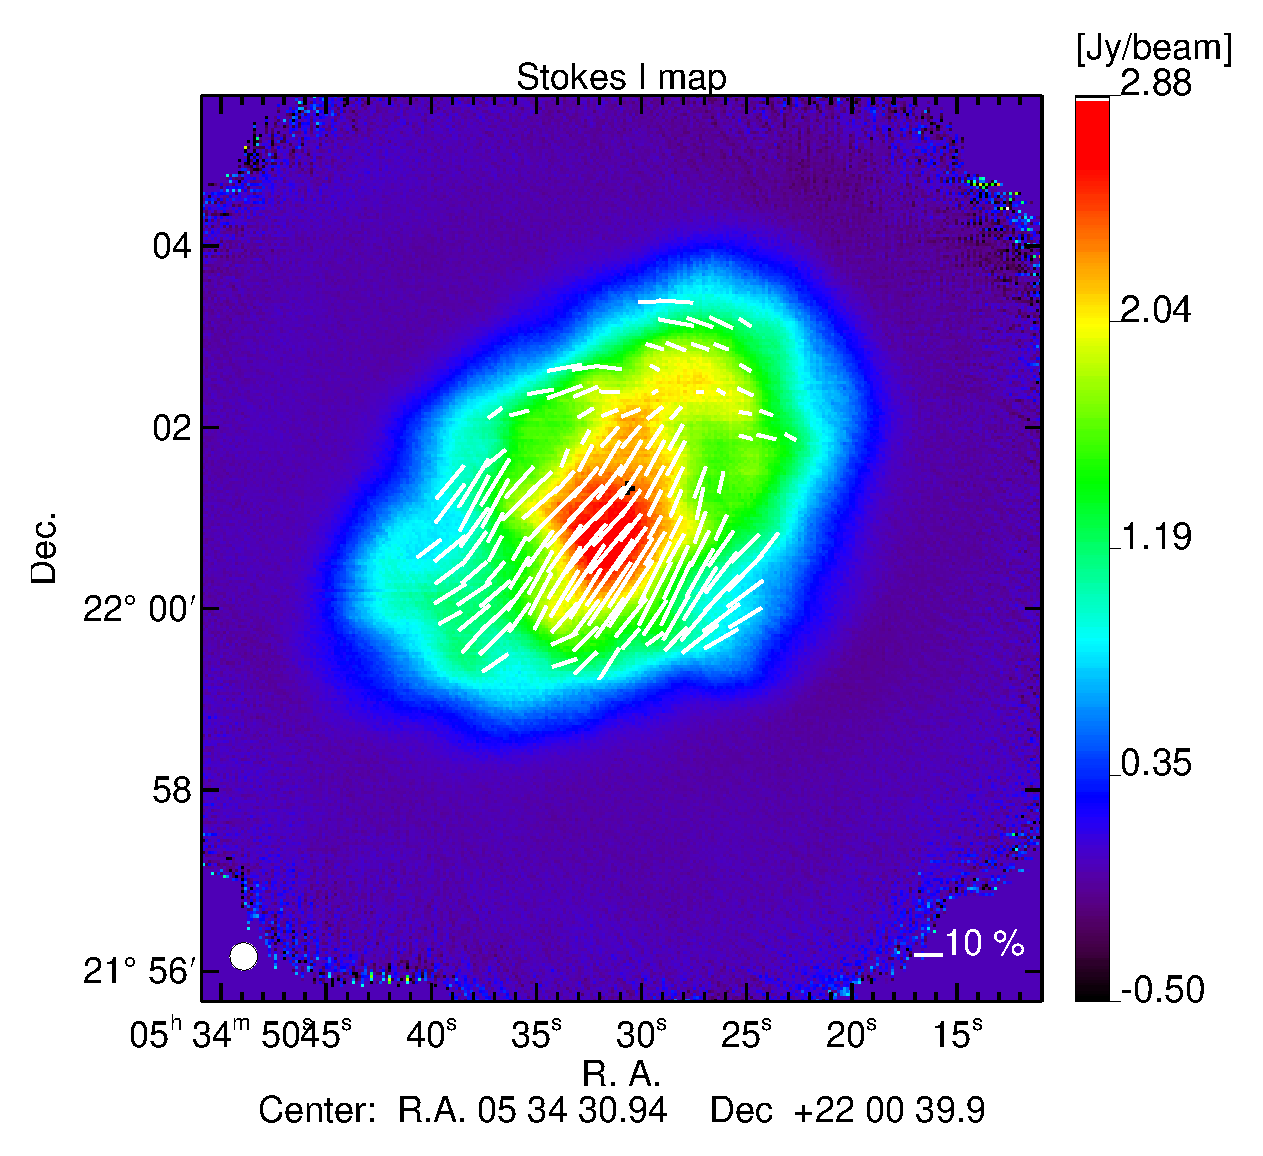
\includegraphics[width=0.32\linewidth,keepaspectratio]{figures/Crab_I_map2_2mm.pdf}}	
	     { 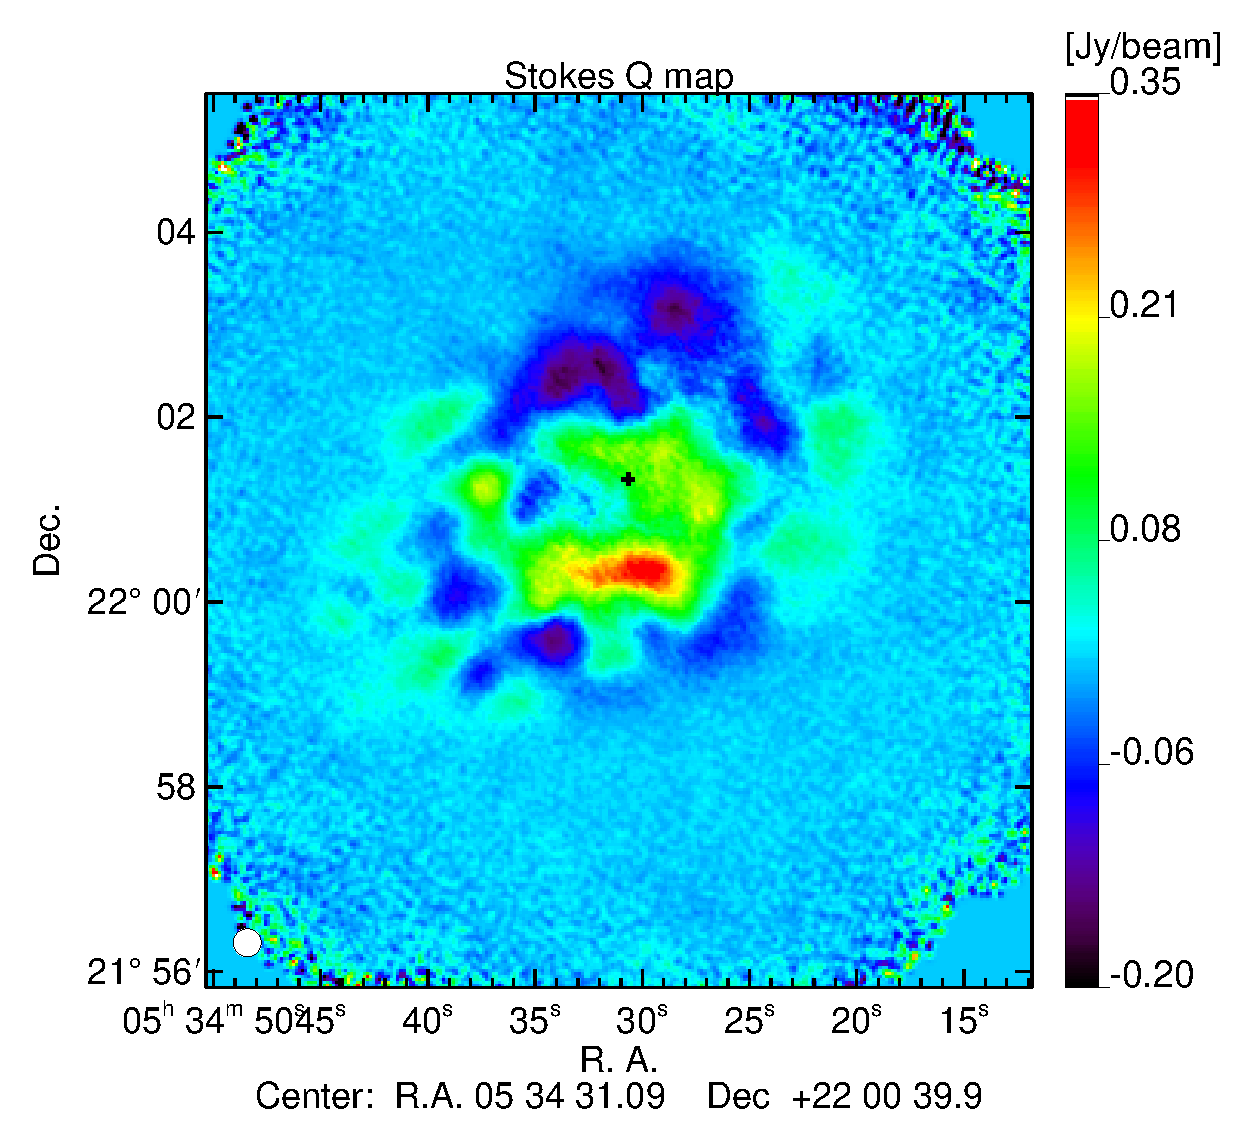
\includegraphics[width=0.32\linewidth,keepaspectratio]{figures/Crab_Q_map2_2mm.pdf}}
          { 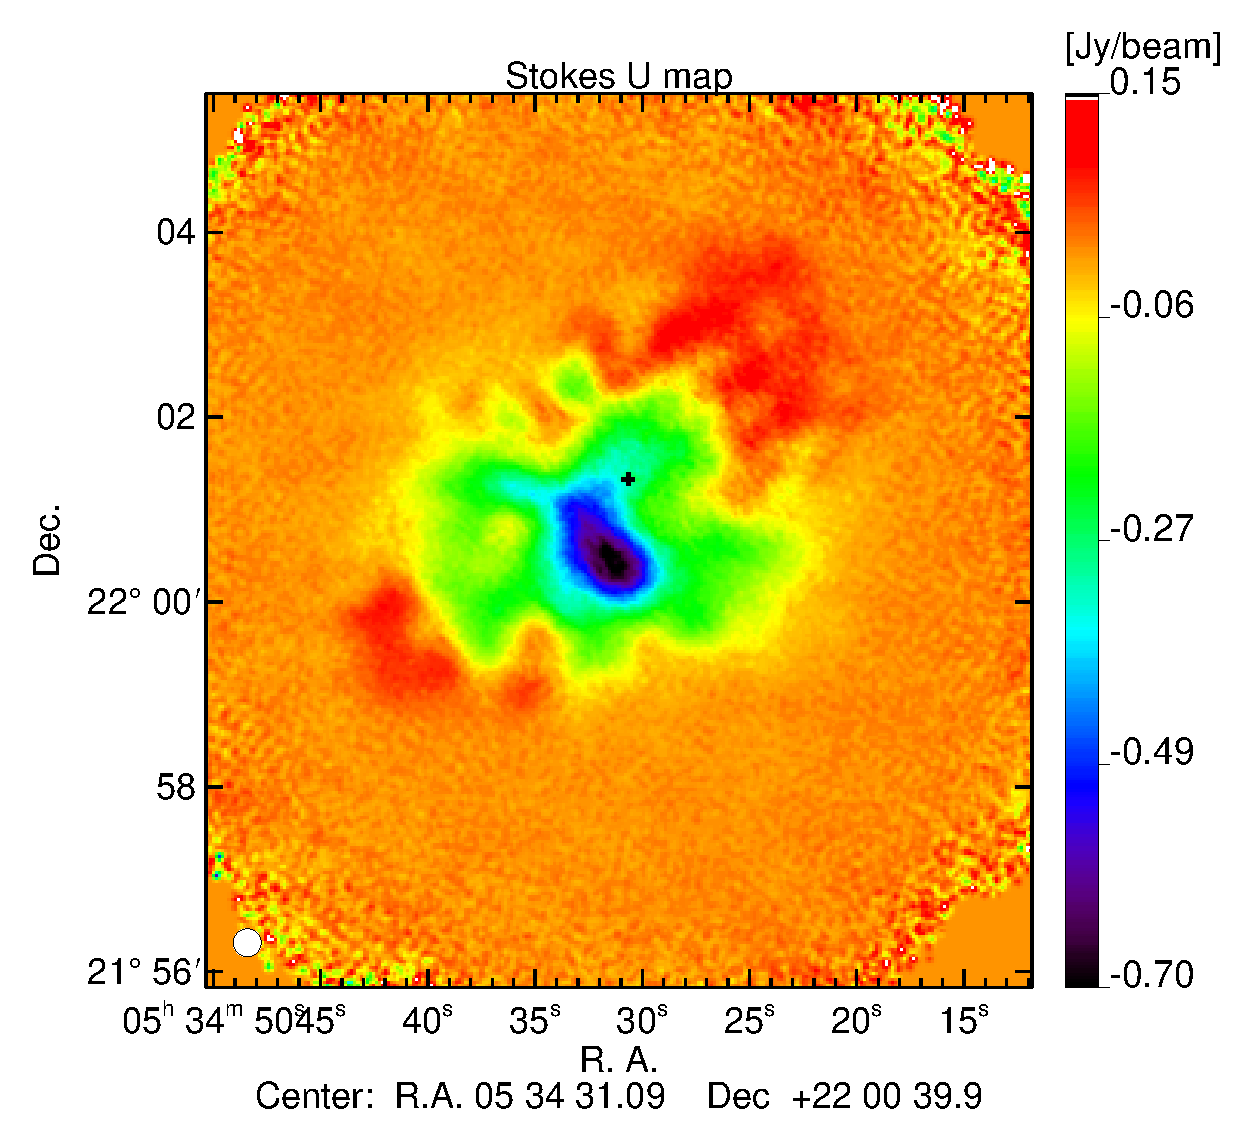
\includegraphics[width=0.32\linewidth,keepaspectratio]{figures/Crab_U_map2_2mm.pdf}} 
           \caption{From left to right: Crab nebula Stokes $I$, $Q$ and, $U$
             maps shown here in Equatorial coordinates obtained at 150 GHz with the \NIKA\ camera. Polarization
             vectors, indicating both the degree and the orientation, are
             over-plotted in white on the intensity map where the polarization
             intensity satisfies $I_{pol} > 3 \sigma_{I_{pol}}$ and $I_{pol} >$ 0.1 Jy. The \NIKA\ FWHM is shown in the lower left.
             The black cross marks the pulsar position.}
\label{crab_intensity_maps}
\end{figure*}


\section{Introduction}\label{sec:introduction}
The polarization of the Cosmic Microwave Background (CMB) anisotropies offers a
powerful way to investigate the early Universe. It can be decomposed into a
scalar and a pseudo-scalar field, respectively called $E$ and $B$ modes. The
primordial density fluctuations (scalar perturbations) can only produce $E$ type
CMB polarization, while $B$ type CMB polarization can only be produced by
primordial (tensor perturbations) gravitational waves
\citep{polnarev1985polarization, 1997PhRvL..78.2054S} arising from the
inflationary epoch \citep{PhysRevD.23.347, linde1982new} and by gravitational
lensing of the $E-$modes (\cite{ade2015planck} and refs. therein).  The
detection of the primordial $B-$modes would set tight constraints on
  Inflation models and constitutes one of the most ambitious goals of modern
observational cosmology.

Recently, \citet{bicepplanck2015,bicep2016} set a 95\% upper limit for the
detection of the tensor to scalar ratio $r$ $\textless$ 0.07.  Upcoming CMB
experiments aiming at measuring the primordial $B-$modes require an accurate
determination of the foreground emissions to the CMB signal and a high control
of systematic effects. One of the most difficult parameters to be characterized
for a CMB polarization experiment is the calibration of residual cross
polarization and of the absolute polarization angle. This can be achieved using
observations of well known polarized sources like the Crab nebula. The Crab
Nebula (or Tau A) is a plerion-type supernova remnant emitting a highly
polarized signal \citep{1978A&A....70..419W,1991ApJ...368..463M}.  The
synchrotron emission from the nebula is observed in the radio frequency domain,
which is powered by a pulsar located at equatorial coordinates (J2000) $R.A. =
5^h34^m32s$ and $Dec. = 22^{\circ}0^{\prime}52^{\prime\prime}$ through its jet.
Moreover, near the center of the nebula one observes a shock, which is formed
where the jet is thermalized and ultra-relativistic particles are released into
the surrounding nebula \citep{2000ApJ...536L..81W,2011A&A...528A..11W}. The Crab
nebula is the most intense polarized astrophysical object in the microwave sky
at angular scales of few arcminutes and for this reason it is of particular
interest for the calibration of CMB polarization experiments, which have
beamwidths comparable to the extension of the source. It is also quite isolated
with low background diffuse emission. For a more detailed review on this source
we refer to \citet{2008ARA&A..46..127H}.

The Crab nebula is used for polarization cross-check analysis in the frequency
range from 30 to 353 GHz \citep{2011ApJS..192...19W,2015arXiv150702058P}. High
angular resolution observations from the XPOL experiment \citep{thum2008} at the
IRAM 30 m telescope have revealed the spatial distribution of the Crab Nebula in
intensity and polarization at 90 GHz with an absolute accuracy of 0.5$^{\circ}$
in the polarization angle \citep{aumont2010}. Such high resolution observations
of the Crab nebula in polarization are crucial for future \NIKAd\ polarization
observations and could be very useful for the calibration of the next generation
of polarization experiments, in particular those aiming at a precise measurement
of the CMB polarization that have a large frequency range to be able to
carefully study and subtract foreground emission \citep{2016IJMPD..2540008K}.

Previous studies \citep{macias2010} of the total Spectral Energy Distribution
(SED) of the Crab nebula have shown a spectrum well described by a single
synchrotron component at radio and mm wavelengths and predict negligible
variations in polarization fraction and angle in the frequency range of interest
for CMB studies.
 
Observations of the polarization of the Crab Nebula have been performed with the
\NIKA\ camera \citep{monfardini2010,catalano2014,monfardini2014} at the IRAM 30
m telescope during the observational campaign of February, 2015. A first
overview of the \NIKA\ Crab polarization observations, focusing on instrumental characterization of the polarization system, was given in
\cite{2016JLTP..184..724R}. In this paper we go a step further in the analysis
by combining \NIKA\ observations with published values at other frequencies to trace the
polarized SED of the Crab nebula. We use polarization observations from the \WMAP\
satellite at 23, 33, 41, 61 and 94 GHz \citep{2011ApJS..192...19W}, from the
\Planck\ satellite at 30, 44, 70, 100, 143, 217, 353 GHz and from XPOL/30m at 90 GHz
\citep{aumont2010}. 

The paper is organized as follows: in Sec.~\ref{sec:NIKA observations} the
intensity and polarization maps obtained with the \NIKA\ camera are presented
together with the polarization degree and angle spatial distributions;
Sec.~\ref{sec:Polarization estimates in CMB experiments like beams} presents the
reconstruction of the polarization properties of the Crab nebula in well defined
regions; Sec.~\ref{sec:Polarization intensity Spectral Energy Density (SED)}
presents the Crab nebula SED in temperature and polarization; in
Sec.~\ref{sec:conclusions} we present our conclusions.
 \begin{figure*}
\centering
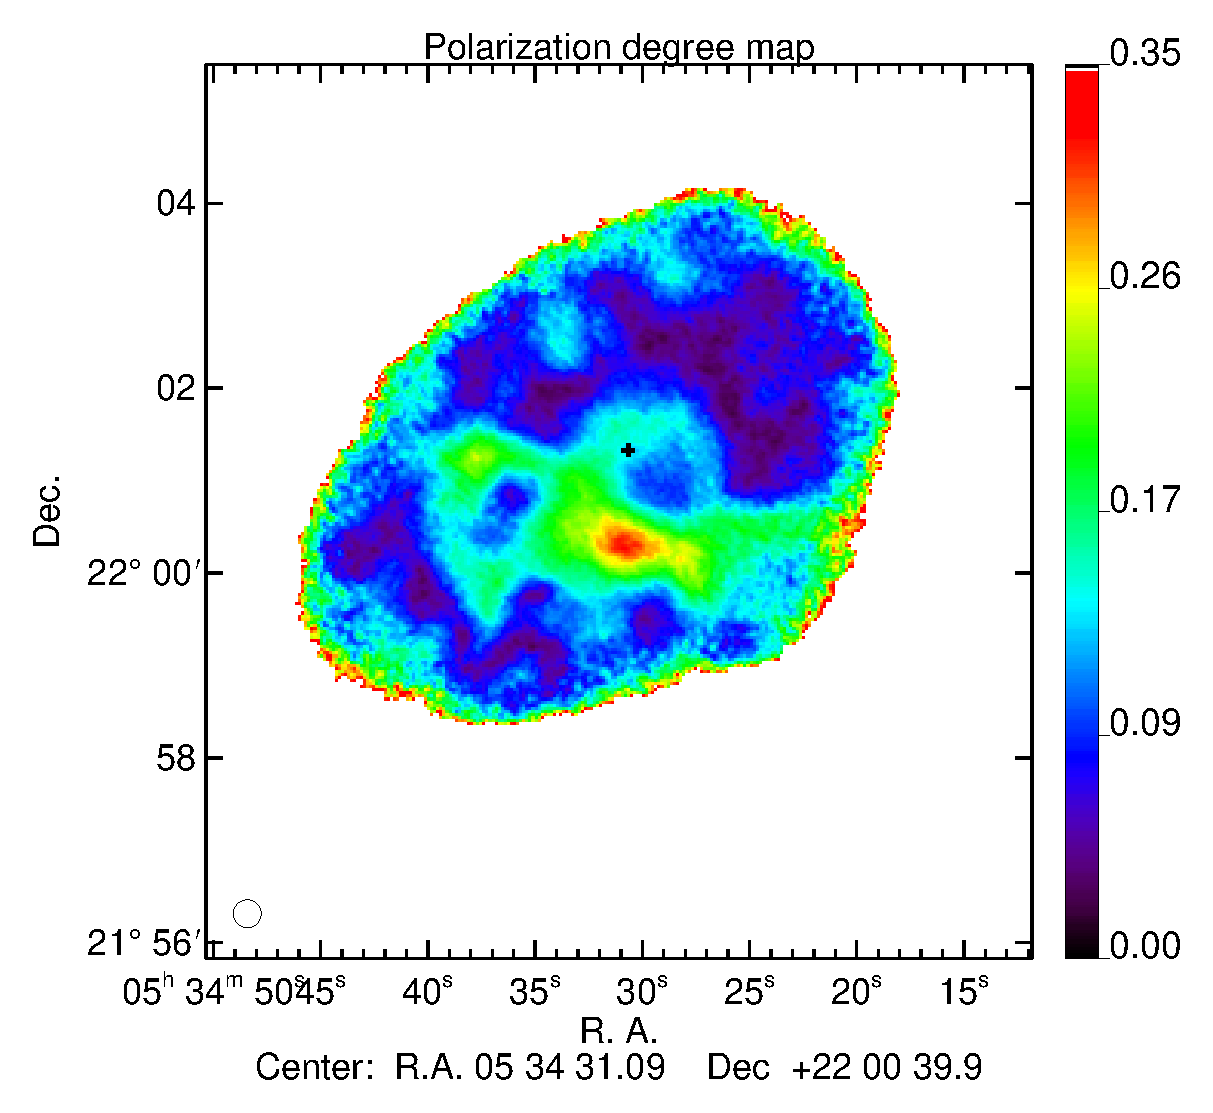
\includegraphics[clip, angle=0, scale = 0.35]{figures/Crab_pol_deg2_2mm.pdf}
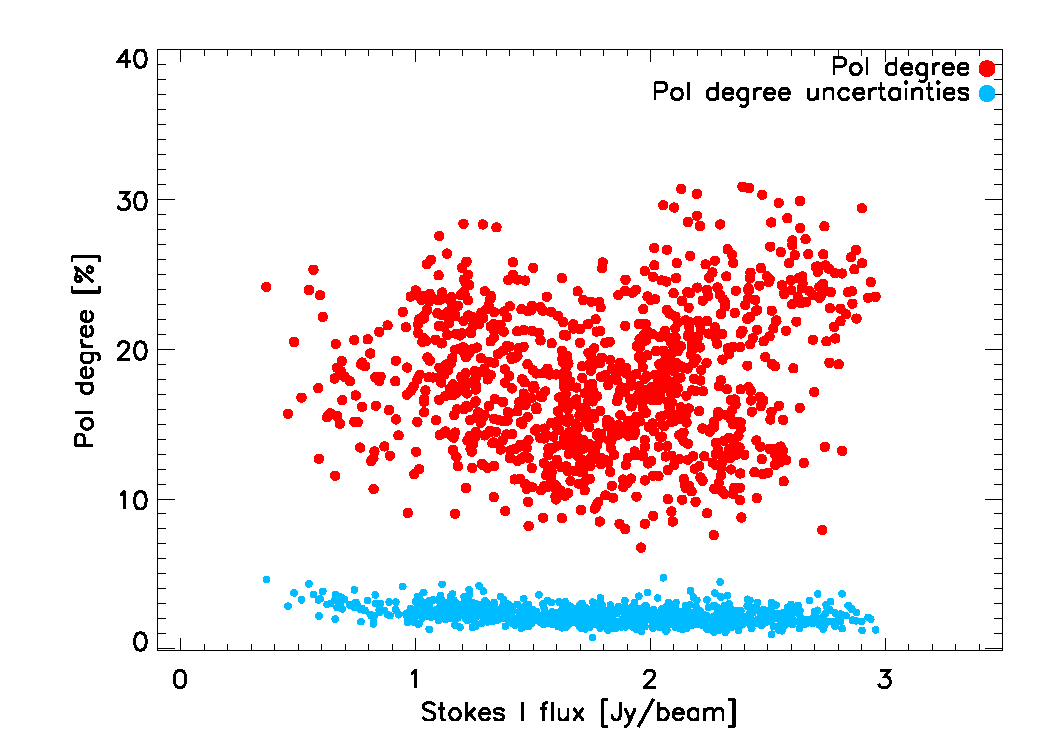
\includegraphics[clip, angle=0, scale = 0.5]{figures/pol_deg_vs_I_2mm.pdf}
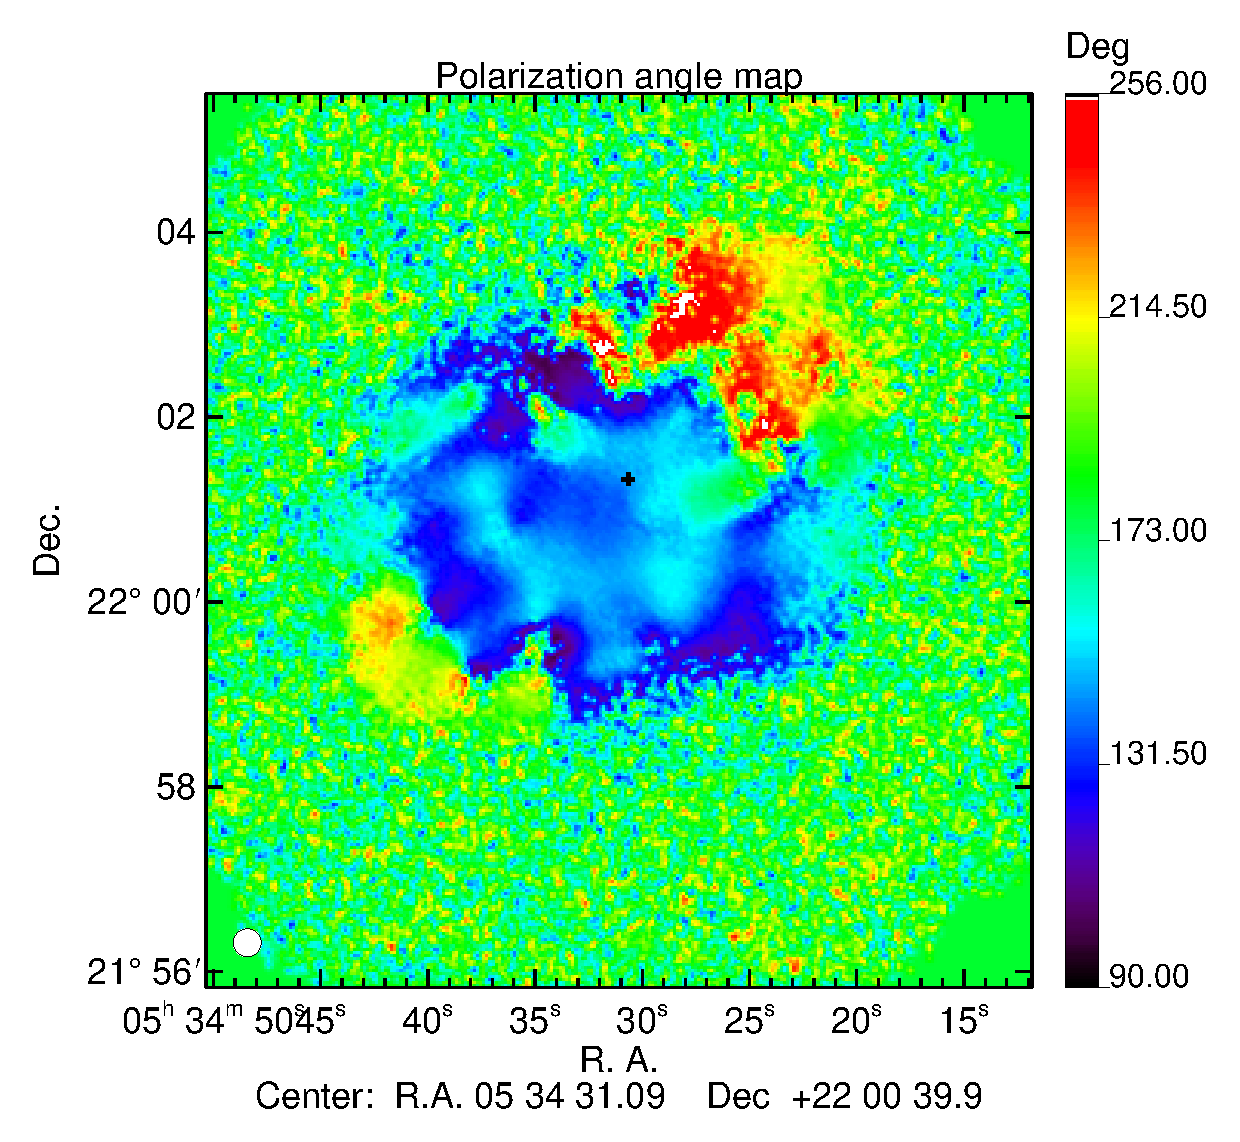
\includegraphics[clip, angle=0, scale = 0.35]{figures/Crab_angle2_2mm.pdf}
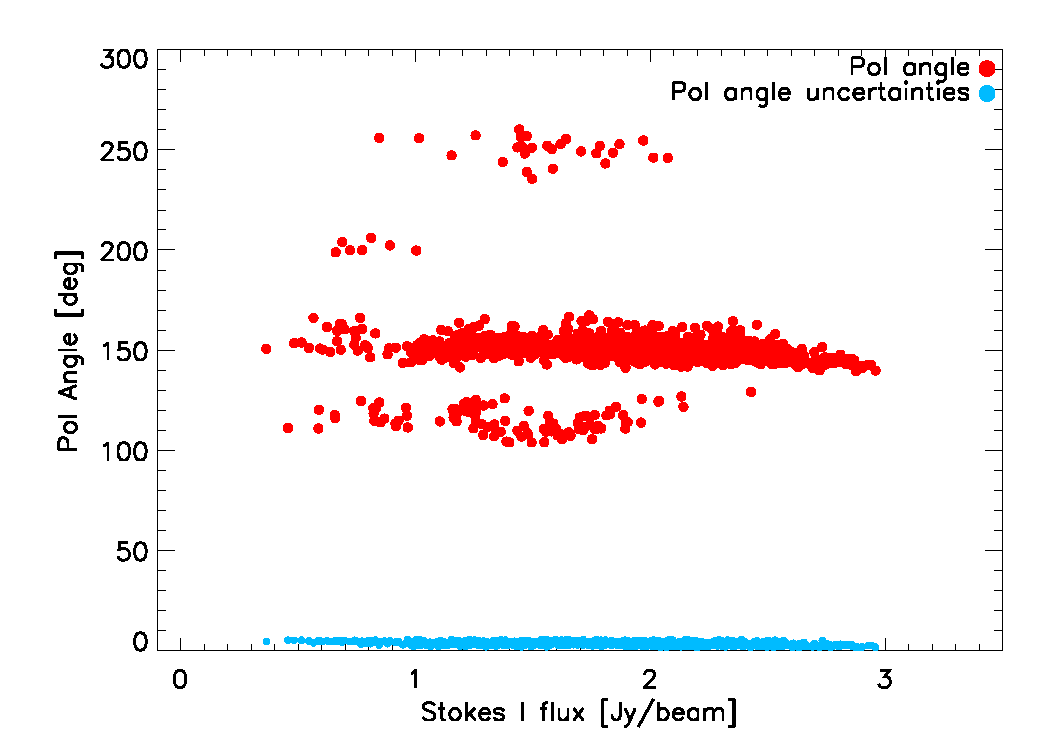
\includegraphics[clip, angle=0, scale = 0.5]{figures/pol_angle_vs_I_2mm.pdf}
\caption{{\it Top}: The left panel shows the polarization
  degree map $p$, uncorrected for noise bias, of the Crab nebula. The right panel shows the noise bias
  corrected $p$ values as a function of total intensity map (Stokes $I$). The
  condition $I_{pol}$ $\textgreater$ 5$\sigma_{I_{pol}}$ is satisfied for those values. {\it
    Bottom}: on the left we present the polarization angle map $\psi$ (Equatorial coordinates system) of the
  Crab nebula. On the right panel the distribution of $\psi$ values is
  represented as a function of the total intensity in the case of very high S/N ratio where $I_{pol}$ $\textgreater$ 5$\sigma_{I_{pol}}$ . The cyan dots represent the uncertainties calculated as the
  dispersion between different observational scans. The black cross marks the pulsar position on the maps.}
\label{fig:pol_degree}
\end{figure*}
 \begin{figure}
  \centering
      {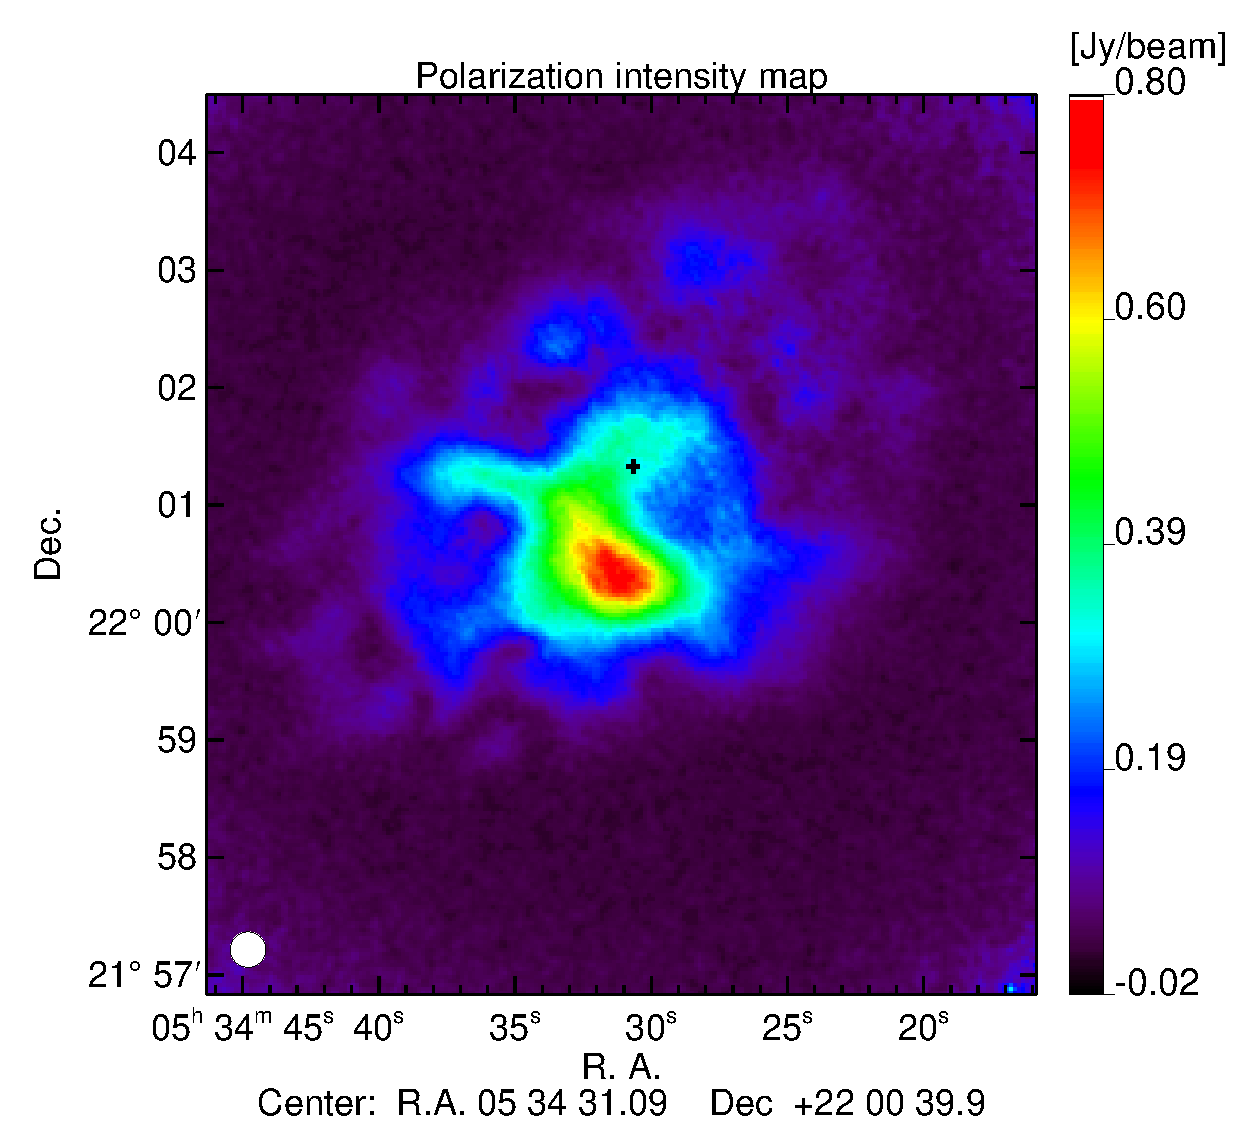
\includegraphics[width=0.75\linewidth,keepaspectratio]{figures/Crab_ipol2_2mm.pdf}}
\caption{\NIKA\ polarized intensity map of the  Crab nebula at 150 GHz. The map shows high polarized emission reaching a value of 0.8 Jy beam$^{-1}$. The telescope beam FWHM is shown in the lower left. The black cross marks the pulsar position.}
\label{crab_ipol_maps}		
  \end{figure}
 

\section{\NIKA\ observations of the Crab Nebula}\label{sec:NIKA observations}
\subsection{\NIKA\ camera and polarization setup}\label{sec:nika camera}
\NIKA\ is a dual band camera observing the sky in intensity and polarization at
150 and 260 GHz with 18~arcsec and 12~arcsec FWHM resolution, respectively. It
has a Field-of-View (FoV) of 1.8$^{\prime}$ at both wavelengths. It was operated at the
IRAM 30~m telescope between 2012 and 2015. A detailed description of the
\NIKA\ camera can be found in \citet{monfardini2010, monfardini2011} and
\citet{catalano2014}.

In addition to having performed intensity observations, \NIKA\ was also a test
bench for the polarization system of the final instrument
\NIKAd\ \citep{calvo2016,catalano2016nika2,2017arXiv170700908A}, which was installed at the
telescope in October, 2015. The polarization setup of \NIKA\ and
\NIKAd\ consists in a continuously rotating a metal mesh half wave plate (HWP)
followed by an analyzer, both at room temperature (for \NIKA) and placed in
front of the entrance window of the cryostat. The Lumped Elements Kinetic
Inductance Detectors (LEKIDs) are not intrinsically sensitive to
polarization. The HWP rotates at 2.98 Hz which modulates the polarization signal
at $4\times 2.98$~Hz. With a typical telescope scanning speed of 26.23 arcsec/s,
this provides a quasi-simultaneous measure of Stokes parameters $I$, $Q$ and $U$
%in Nasmyth coordinates ({\it i.e.} cabin reference coordinates)
per beam and
places the polarized power in the frequency domain far from the low frequency
electronic noise and the atmospheric fluctuations. \cite{ritacco2017} gives more
details on the \NIKA\ polarization capabilities and describes the performance of
the instrument at the telescope. In particular the sensitivity of the
\NIKA\ camera in polarization mode was estimated to be 50 mJy.$s^{1/2}$ at 150
GHz.

\NIKA\ has provided the first polarization
observations performed with Kinetic Inductance Detectors, confirming that KIDs are a
suitable detector technology for the development of the next generation of CMB
experiments.
%Unfortunately, the observations of the Crab nebula performed at 260 GHz have been limited by the sensitivity of the \NIKA\ instrument in polarization and the resulting maps show a no significant detection, for that reason here we discuss only the observations performed at 150 GHz. 

\subsection{\NIKA\ observations}\label{sec:nika_observations}
%Polarization measurements with the \NIKA\ camera have been carried out with a combined action of a continuously rotating metal-mesh Half Wave %Plate (HWP), a polarizer and KIDs arrays mounted inside the \NIKA\ instrument. 
%Since \NIKA\ detectors \citep{roesch2012} are not sensitive to the linear polarization a polarizer is necessary to select one direction of it. 
Crab nebula polarization observations with the \NIKA\ camera were performed at
the IRAM 30~m telescope in February, 2015. The average effective opacity at 150 GHz was $\tau$ = 0.2.  Fig.~\ref{crab_intensity_maps} shows
the Stokes $I$, $Q$ and $U$ maps obtained by a co-addition of 16 maps
of $8 \times 6$ arcminutes for a total observation time of $\sim$ 2.7 hours. The
maps were performed in equatorial coordinates in four different scan
directions: 0$^{\circ}$, 90$^{\circ}$, 120$^{\circ}$, 150$^{\circ}$. This
allowed us to have the best coverage of the source.% and to reduce filtering effects.

To obtain the Stokes $I$, $Q$, and $U$ Crab nebula maps in Equatorial coordinates, we have used a dedicated
polarization data reduction pipeline \citep{ritacco2017}, which is an extension
of the intensity \NIKA\ pipeline \citep{catalano2014,adam2013}. The main steps
of the polarization pipeline are summarized below:
\begin{enumerate}
\item  Subtraction of the HWP induced parasitic signal, which is modulated at harmonics of the HWP rotation frequency and represents the most tedious noise contributing to the polarized signal. 
\item Reconstruction of the Stokes $I$, $Q$ and $U$ time ordered information
  (TOI) from the raw modulated data. This is achieved using a demodulation
  procedure consisting in a lock-in around the fourth harmonic of the HWP rotation frequency, where the polarization signal is located.
\item Subtraction of the atmospheric emission in the demodulated TOIs using
  decorrelation algorithms. In polarization, the HWP modulation reduces
  significantly the atmospheric contamination and there is no need to
    further decorrelate the $Q$ and $U$ TOI's from residual atmosphere. By contrast, in
  intensity the atmospheric emission fully dominates the signal and to recover
  the large angular scales we use the 260~GHz band as an atmosphere
  dominated band like in \cite{adam2013}.  This decorrelation impacts the
    reconstructed Stokes maps via a transfer function. We have estimated this function
    with simulated observations of diffuse emission that were passed through the
    data reduction pipeline, with the exact same scanning, sample flagging and data
    processing as real data. We found that the power spectrum of the output maps
    match that of the input one to better than 1\% (resp.~5\%) on scales smaller
    (resp.~larger) than $\sim 1'$. The impact of the data processing is thus
    negligible compared to uncertainties on absolute calibration on small
    scales, and its moderate effect on large angular scales is further reduced
    with the subtraction of a zero level for the photometry (see below). In the
    following, we therefore neglect this transfer function.


\item Correction of the intensity-to-polarization-leakage-effect, which was
  identified in observations of unpolarized sources like the planet Uranus. For
  point sources the effect was about 3\% peak-to-peak, while for extended sources like the Crab nebula it has been found to be the order of 0.5 \% peak-to-peak. 
  \cite{ritacco2017} describes the algorithm of leakage correction developed specifically for \NIKA\ polarization observations. Applying this algorithm to Uranus observations the instrumental polarization is reduced to 0.6\% of the total intensity $I$.
  \item Projection of the demodulated and decorrelated Stokes $I$, $Q$, and $U$ TOIs into Stokes $I$, $Q$ and $U$ equatorial coordinates maps.

\end{enumerate}

\subsection{Crab polarization properties}\label{sec:pol_properties}
In this section we discuss the polarization properties of the source in terms of polarization degree $p$ and angle $\psi$, which are defined through the Stokes parameters $I, Q$, and $U$ as follows:
\begin{equation}
 p    = \frac{\sqrt{Q^2 + U^2}}{I} \nonumber 
\end{equation}
and
 \begin{equation}
 \psi = \frac{1}{2}\arctan\frac{U}{Q}.\label{angledegree_polar}
 \end{equation}
These definitions are not linear in $I$, $Q$ and $U$ and therefore, the observational uncertainties have to be carefully considered, {\it i.e.} p, $\psi$ are noise biased. 
\citet{1980A&A....91...97S,1985A&A...142..100S,montier} proposed analytical solutions to correct for this bias. For intermediate and high S/N ratio the polarization degree and its uncertainty read:
 \begin{eqnarray}
 p    &=& \frac{\sqrt{Q^2 + U^2 - \sigma_{Q}^2 - \sigma_{U}^2}}{I}, \nonumber \\ 
  \sigma_{p} &=& \frac{\sqrt{Q^2\sigma_Q^2 + U^2\sigma_U^2 + p^4I^2\sigma_I^2}}{pI^2}.
  \label{p_true_degree}
 \end{eqnarray}
 Furthermore, the polarization angle in a high S/N regime can be approximated by Eq.~\ref{angledegree_polar} with the uncertainty
  \begin{eqnarray}\label{angle_uncertainty}
  \sigma_{\psi} = \frac{\sqrt{Q^2\sigma_Q^2 + U^2\sigma_U^2}}{2(pI)^2}.
  \end{eqnarray}

The angular distribution map of the polarization degree $p$ of the Crab nebula
without noise bias correction is presented on the top left panel of
Fig.~\ref{fig:pol_degree}.  Tab.~\ref{tab:crab_comparison} presents the total
flux $I$, polarization degree $p$ and angle $\psi$ computed on the pulsar
position, highlighted by a black cross on maps, and the Stokes $I$ peak
position.  The polarization degree $p$ reaches a value of 22.5 $\pm$0.7 \% at
the peak of the total intensity, which is consistent with what we observe on the
top right panel of Fig.~\ref{fig:pol_degree}, where the variation of $p$ as a
function of the Stokes $I$ is shown.  Here the $p$ values have been noise bias
corrected and satisfy the condition $I_{pol}=\sqrt{Q^2+U^2}$ $\textgreater$ 5
$\sigma_{I_{pol}}$. The distribution of the polarization degree appears highly
dispersed around a mean value of 20\%.  The compatibility between the $p$ value
computed at the Stokes $I$ peak position and the above mentioned plot is
expected because we use a very high S/N ratio threshold of 5 $\sigma_{I_{pol}}$,
which restricts the measurement to a small region around the peak of the source.
In addition, the $p$ value found is also consistent within the error bars with
POLKA experiment measurement \citep{2014PASP..126.1027W} (cf.~Table~\ref{tab:crab_comparison}).

The polarization degree decreases towards the edges of the
source. Furthermore, the high polarization degree observed at the extremities of the source is misleading and caused by the very low S/N ratio of the Stokes $I$ map observed in these regions. The variation of $p$ highlights the interest of high resolution polarization
observations of the Crab nebula. 

The bottom left panel of Fig.~\ref{fig:pol_degree} shows the spatial distribution of polarization angle
$\psi$.  We observe a relatively constant polarization
angle of about 150 $^{\circ}$ represented here in equatorial coordinates, except
for the northern region where the averaged angle is around $220^{\circ}$, and
some inner regions with lower polarization angle.  These values are confirmed by
the bottom right panel that shows the polarization angle distribution as a
function of total intensity satisfying the condition $I_{pol} > 5\sigma_{I_{pol}}$.

The sudden change of polarization angle on the northern region was already
observed by the XPOL experiment at 90 GHz \citep{aumont2010}.  This together
with the variation of the polarization fraction discussed above confirms the
need of high angular resolution observations at low and high frequencies for a
good understanding of the Crab polarized emission properties.
High resolution observations gives the possibility to compare to all CMB experiments as there are significant polarization fraction variations across the source.

We present in Fig.~\ref{crab_ipol_maps} the 150 GHz Crab polarization intensity
map $I_{pol}$ uncorrected for noise bias. We observe a peak at 0.8 Jy beam$^{-1}$ and the polarization
decreases towards the edges of the nebula.

\section{Total intensity and polarization fluxes}\label{sec:Polarization estimates in CMB experiments like beams}
We compute the total flux across the Crab nebula, which has an extent of about
5$^{\prime}$x7$^{\prime}$ as shown in Fig.~\ref{crab_intensity_maps}.  We use
standard aperture photometry techniques to calculate the flux as shown in
Fig.~\ref{crab_integrated_flux}. We use as center position the center of the
map. A zero level in the map, calculated as the mean of the signal measured on
an external annular ring region (see bottom panel of
Fig.~\ref{crab_integrated_flux}) of radius 4$^\prime$ $\textless$ R $\textless$
4.5$^\prime$, has been subtracted from the map. The total signal estimated is
204.4$\pm$7.9$\pm$10.2 Jy. The first uncertainty term accounts for statistical
uncertainties computed from fluctuations of the signal at large radii.

We use Uranus for absolute point source flux calibration. The flux of the planet is estimated from a frequency dependent model of the planet brightness temperature as described in \cite{moreno2010}. 
This model is integrated over the \NIKA\ bandpasses for each channel, and it is assumed to be accurate at the 5\% level. The final absolute calibration factor is obtained by fitting the amplitude of a Gaussian function of fixed angular size on the reconstructed maps of Uranus, which represents the main beam. For the polarization observational campaign of February 2015 this uncertainty is estimated to be 5\% for the \NIKA\ 2.05 mm channel (150 GHz) \citep{ritacco2017}. 
Nevertheless, as described in \cite{adam2013, catalano2014}, by integrating the Uranus flux up to 100 arcsec, we observe that the total solid angle covered by the beam is larger than the Gaussian best-fit of the main beam by a factor of 28\%. As consequence we account for this factor in the estimation of the fluxes.
Moreover, \cite{adam2013} estimated the uncertainty on the solid angle of the main beam to be 4\%.
Finally, the overall calibration error is estimated to be about 10\%, by considering also the uncertainties on the side lobes.

The polarization efficiency factor estimated across the \NIKA\ 2.05 mm spectral band and reported in \cite{ritacco2017} is $\rho_{pol}$ = 0.9941 $\pm$ 0.0002. This very small efficiency lost of 0.6 \% has a very small impact on the estimation of the polarization fluxes and the calibration error itself. 

\begin{figure}[h!]
  \centering
  \includegraphics[width=0.7\linewidth,keepaspectratio]{figures/Crab_transfer_func.eps}
  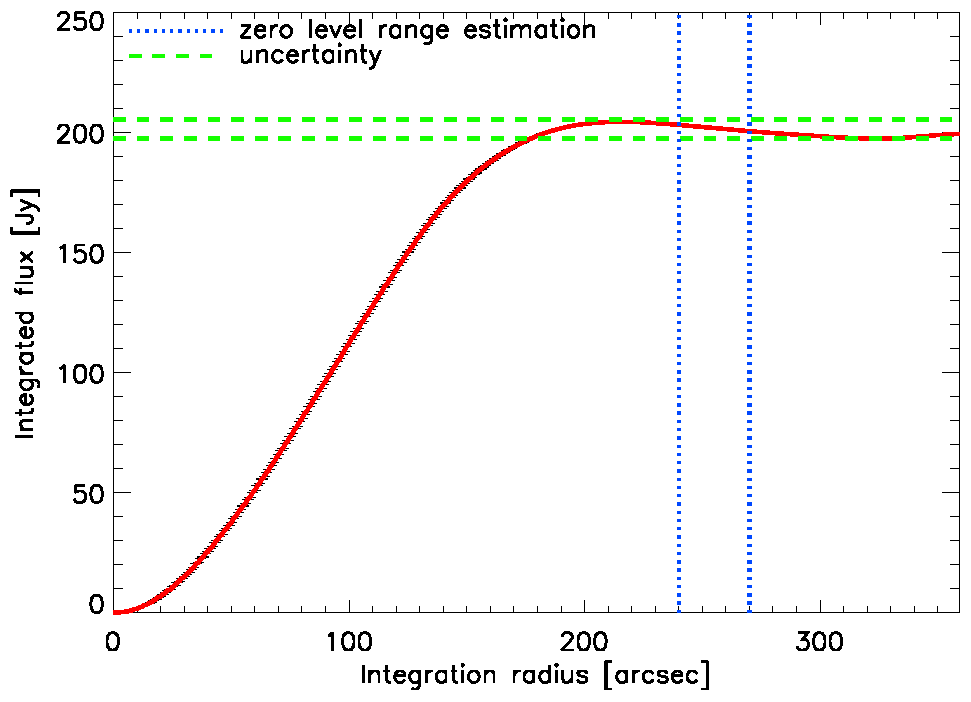
\includegraphics[width=0.7\linewidth,keepaspectratio]{figures/Crab_integrated_flux_2mm.pdf}
  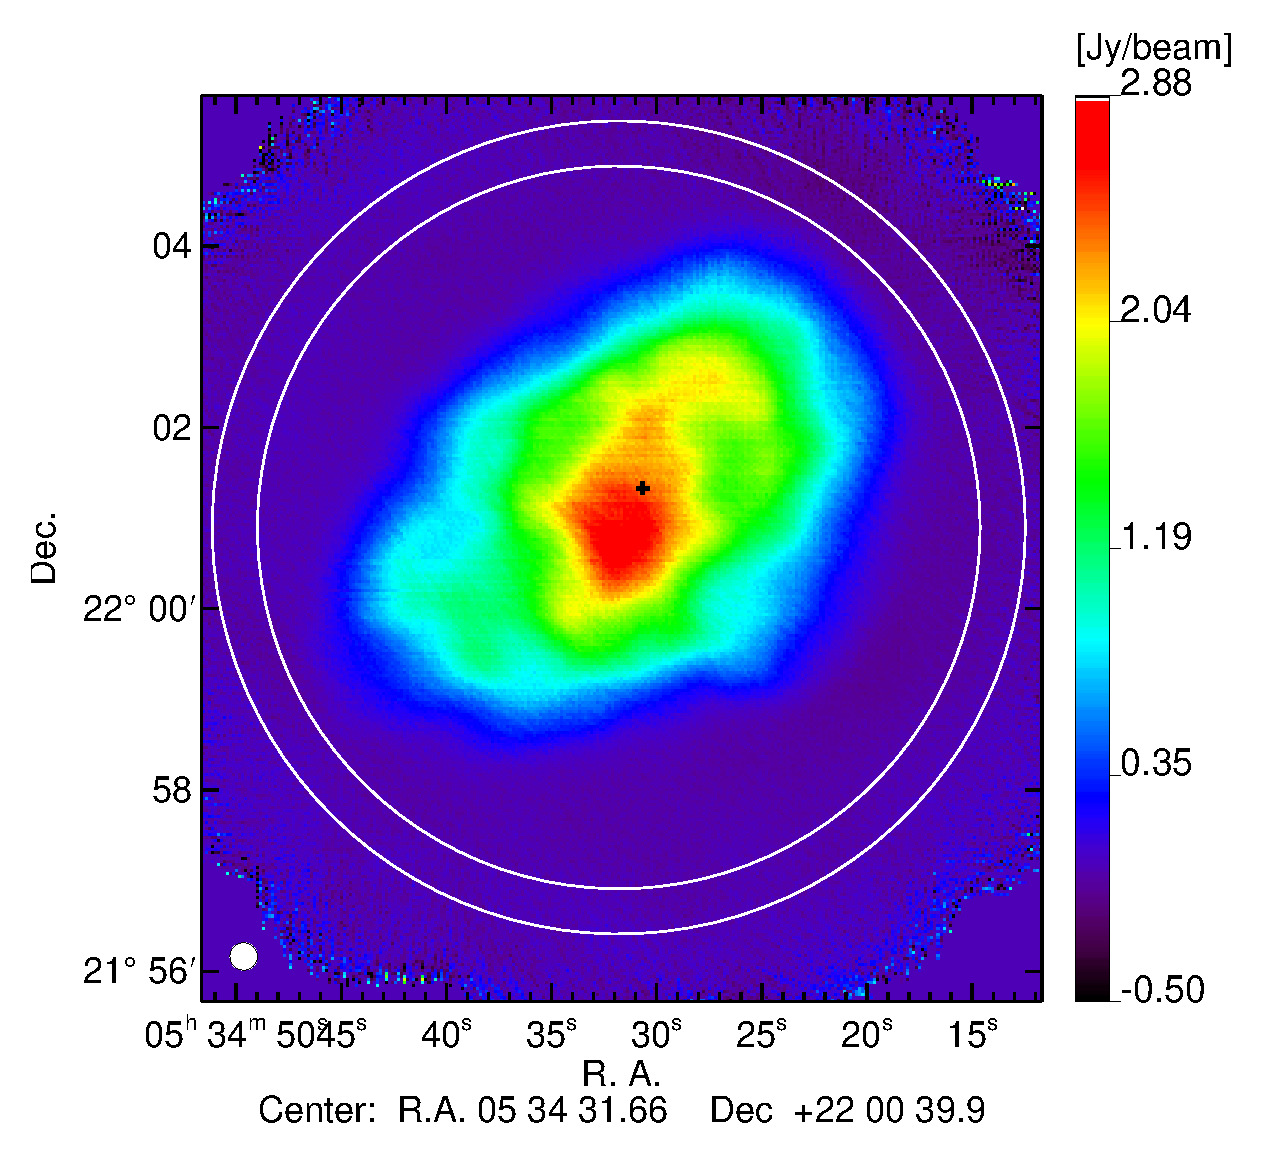
\includegraphics[width=0.8\linewidth,keepaspectratio]{figures/Crab_I_map2_2mm_ring.pdf}
     \caption{Top: Transfer function of the intensity data processing. Middle:
       Cumulative flux of the Crab nebula (top) obtained at 150 GHz over
       4$^{\prime}$ from the center obtained by aperture photometry. The flux
       has been corrected by a zero level in the map, which corresponds to the
       mean of the signal calculated in an annular ring as indicated by the
       white circles on the map (bottom) and by the blue dotted lines on the
       top. The green dotted line represents the uncertainties measured at large
       radii.}
\label{crab_integrated_flux}
\end{figure}

In order to compare our results with low angular resolution CMB experiments, we present in Tab.~\ref{tab:crab_results} the
polarization degree $p$ and angle $\psi$ integrated values obtained in well
defined regions: 5$^\prime$, 7$^\prime$ FWHM from the center of the maps, at the pulsar position and Stokes $I$ peak position.


The polarization angles are here presented in Galactic coordinates to ease the comparison with the \Planck\ \citep{2015arXiv150702058P} and \WMAP\ CMB experiments \citep{2011ApJS..192...19W} and also in Equatorial coordinates within parenthesis.
As discussed in \cite{ritacco2017} a 1.8$^{\circ}$ uncertainty must be considered because the mechanical motor, in which the HWP is mounted, completes 100 steps per tour of the HWP. Therefore, it is the precision associated to the determination of the HWP zero, corresponding to its optical axis in the cabin reference frame.

Notice that the \Planck\ satellite FWHMs are: 33$^{\prime}$, 24$^{\prime}$, 14$^{\prime}$, 10$^{\prime}$, 7.1$^{\prime}$, 5.5$^{\prime}$, 5$^{\prime}$ arcminutes at 30, 44, 70, 100, 143, 217, 353 GHz, respectively.
\WMAP\ satellite has FWHMs: 0.93$^{\circ}$, 0.68$^{\circ}$, 0.53$^{\circ}$, 0.35$^{\circ}$, \textless 0.23$^{\circ}$ at 22 GHz, 30 GHz, 40 GHz, 60 GHz, 90 GHz respectively. 

As stated in \ref{sec:pol_properties}, we use simple Gaussian
  estimators in this work that are unbiased only at high S/N ratio. This adds an
  additional uncertainty on the determination of the degree of polarization $p$
  and on the angle $\psi$ when the SNR is not larger than $\sim 3\sigma$. While
  we can delimit regions of the map as a function of their SNR to give reliable
  results per pixel, the determination of average quantities over the entire map
  is more delicate. Intensity does not suffer from this limitation, so the
  average flux of the source can safely be integrated over all pixels. Taking
  the entire map and averaging it over Gaussian beams of 5$^{\prime}$ and
  7$^{\prime}$ FWHM, we find $\psi = -83.6912 \pm 0.0004^{\circ}$ and $\psi =
  -83.6491 \pm 0.0004^{\circ}$ respectively, while we find $-87.15 \pm 0.04$ and
  $-87.14 \pm 0.07$ if we consider only pixels with a $I_{pol}$ SNR larger than
  3. In terms of polarization degree, we find $p = 8.1 \pm 5\times 10^{-5}\%$
  and $p = 7.5 \pm 4\times 10^{-5}\%$ if we take all the pixels to average $Q$
  and $U$ over our fiducial beams of 5$^{\prime}$ and 7$^{\prime}$,
  respectively, and $p = 6.96 \pm 0.02\%$ and $p = 6.93 \pm 0.06\%$ if we
  restrict our estimation of $Q$ and $U$ to pixels with an $I_{pol}$ SNR larger
  than 3.  An additional uncertainty at a level of 1$\%$ on
  $p$ and $4^{\circ}$ on $\psi$ should be considered at this stage to account
  for the yet incomplete subtraction of the noise bias on polarized quantities.


Fig.~\ref{crab_p_angle_comparison} shows the polarization fraction (top) and polarization angle (bottom) of the Crab nebula as a function of the frequency as measured by
five different instruments: \Planck\ \citep{2015arXiv150702058P},
\WMAP\ \citep{2011ApJS..192...19W}, XPOL \citep{aumont2010} and \NIKA\ (this paper).  

The solid line in both figures represents the weighted-average found using all
the observations shown and the dashed lines represent the uncertainties
estimated on the weighted-average. Considering only low frequency data
(\textless 200 GHz) and excluding the XPOL data (see below) we find that the
degree of polarization of the Crab nebula at arcmin scales is 7.1$\pm$0.1 \%.
In terms of degree of polarization most data sets are consistent at the
2$\sigma$ level with the weighted-average value. For XPOL the discrepancy can
probably be explained by the lower sensitivity of the single channel XPOL
experiment to the lower than average polarization of the outer parts of the
nebula.

In the case of \Planck\, the observed discrepancy at high frequency could be due
to an evolution of the Crab nebula polarization properties with frequency, but
this hypothesis is disfavored by the polarization angle measurements that seem
to be consistent with the mean value across all frequencies.

The weighted-average of the polarization angle of the Crab nebula at $\geq$ 5$^{\prime}$ scales is therefore estimated considering all available observations, is -88.1$^{\circ}$
$\pm$ 0.3.  All the observations shown on the bottom panel of
Fig.~\ref{angledegree_polar} agree within 1$\sigma$ with this value except for
the \Planck\ value at 30 GHz, which is slightly high.

\begin{table*}
  \centering
      \begin{tabular}{ccccccccc}
      \hline
      \hline
       & $I$ [Jy] & $I_{pol}$ [Jy] & $p$ [\%] &  $\psi$ [$^\circ$] &\\      
      &  &  &  & & I$_{pol}$ $>$ 3$\sigma_{I_{pol}}$ \\
      \hline
 %seen by 7$^{\prime}$   & 231.8$\pm$0.2  & 14.03$\pm$0.09 & 6.05$\pm$0.04 & -85.1$\pm$0.5$\pm$1.8(syst)  \\ 
    7$^{\prime}$ FWHM centered   & 207.9$\pm$0.3  & 14.4$\pm$0.1 & 6.93$\pm$0.06 & -83.4 (141.02)$\pm$0.2 & -87.14 (144.8)$\pm$0.07$\pm$1.8$^*$\\ 
 
%            seen by 5$^{\prime}$ & 219.0$\pm$0.1  & 14.8 $\pm$0.03 & 6.78$\pm$0.01 & -83.7$\pm$0.1$\pm$1.8(syst)    \\ 
    5$^{\prime}$ FWHM centered & 207.2$\pm$0.1  & 14.4 $\pm$0.04 & 6.96$\pm$0.02 & -82.3 (139.9)$\pm$0.7 & -87.15 (144.8)$\pm$0.04$\pm$1.8$^*$ \\ 
  %    P $\textgreater$ 3 $\sigma_P$     & 84.6$\pm$0.01  & 10.51 $\pm$0.01 &12.42$\pm$0.01 & -87.15 $\pm$0.04$\pm$1.8(syst) \\
     	      
              %FWHM = 1.4$^{\prime}$ around polarization intensity peak where I$_{pol}$ $\textgreater$ 0.2 Jy& 60.6$\pm$0.2 & 10.28$\pm$0.01  & 16.96$\pm$0.01 &-87.69$\pm$0.01$\pm$1.8(syst)\\
              
             
                \hline            
    \hline   
    \end{tabular}
   \caption{ 
   	*A systematic angle uncertainty of 1.8$^{\circ}$ must be considered in the polarization angle error budget.
   	 Total flux $I$, polarized intensity flux $I_{pol}$,
     polarization degree $p$, and angle $\psi$. The values have been calculated within 7$^{\prime}$ and 5$^{\prime}$ radius from the center of the map. The polarization angle has been also calculated where I$_{pol}$ $\textgreater$ 3$\sigma_{I_{pol}}$ to avoid the contribution of pixels biased by the noise.
     The polarization angle is here given in Galactic coordinates and in Equatorial coordinates within parenthesis. 
     An total calibration error of 10 $\%$ must be accounted for and propagated to the
     polarization estimates.
   %The values measured in two regions with high S/N ratio are also presented.
    }
    \label{tab:crab_results}
 \end{table*}
 
 \begin{table*}
  \centering
      \begin{tabular}{ccccccccc}
      \hline
      \hline
      & &  Pulsar & & \\
       & $I$ [Jy]& $p$ [\%] & $\psi$ [$^\circ$] & \\ 
       \hline
      POLKA & 1.63 & 25.3 $\pm$ 3.0 & 145.1 $\pm$ 3.3 & \\
      XPOL  & & 13.9 $\pm$ 0.6 & 158.1 $\pm$ 0.5 &  \\
      SCUPOL & & 14.3 $\pm$ 1.8 & 140.0 $\pm$ 2.8& \\
      \hline
      \hline
       & &  Peak & & \\
       \hline
      POLKA & 1.72 & 25.0 $\pm$ 3.1 & 151.7 $\pm$ 3.5 &  \\
      XPOL  & & 25 & 149.0 $\pm $ 1.4 &  \\
      SCUPOL & & 18.7 $\pm$ 1.5 & 146.1 $\pm$ 2.1&\\
  
     \hline            
    \hline   
    \end{tabular}
   \caption{ 
   	%Total flux $I$, polarization degree $p$, and angle $\psi$ estimated at the pulsar position evidenced on the maps by a black cross and at the peak of the Stokes $I$ map. The polarization angle is here given in Equatorial coordinates and in Galactic coordinates within parenthesis.
   	Values estimated by POLKA, XPOL, SCUPOL reported in \cite{2014PASP..126.1027W} at the pulsar and peak position, respectively. 
    }
    \label{tab:crab_comparison}
 \end{table*}


\begin{table*}
  \centering
      \begin{tabular}{ccccccccc}
      \hline
      \hline 
   & $I$ & $Q$ & $U$ & $I_{pol}$ & $p$ & $\psi$ & \\ 
      &	[Jy] & [Jy] & [Jy] & [Jy] & [\%] &[$^\circ$] & \\
       \hline
	Peak \\	
	\hline
  A pixel beam size &  0.219 $\pm$ 0.001 & 0.0053 $\pm$ 0.0047 & -0.045 $\pm$ 0.001 & 0.045 $\pm$ 0.001 & 20.7 $\pm$ 0.7 & 138.3 $\pm$ 2.3 $\pm$ 1.8 & \\
 	\hline
  \NIKA\ beam size & 8.28 $\pm$ 0.12 & 0.31 $\pm$ 0.06 & -1.70 $\pm$ 0.05 & 1.73 $\pm$ 0.05 & 20.9 $\pm$ 0.8 & 140.20 $\pm$ 0.04 $\pm$ 1.8 & \\	
     \hline            
    \hline   
    \end{tabular}
   \caption{ 
   	Flux densities in total power, polarization and polarization properties estimated at the peak position of the Stokes $I$ map, which position is shown on the maps with a black cross. The polarization angle is here given in Equatorial coordinates and in Galactic coordinates within parenthesis.}
    \label{tab:crab_comparison}
 \end{table*}



  

\begin{figure}
  \centering
          { 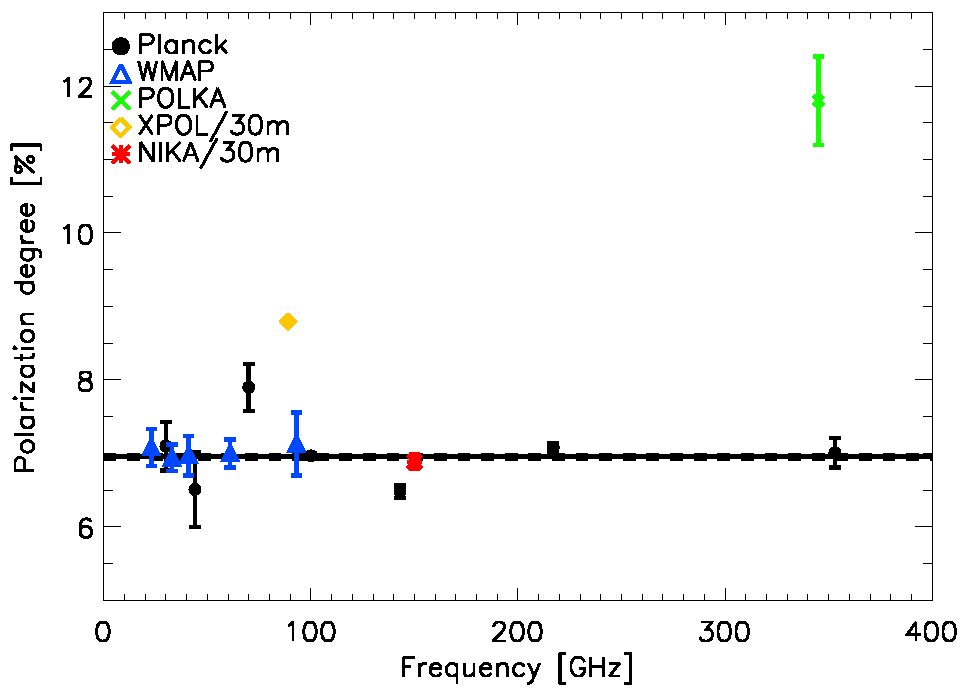
\includegraphics[width=1\linewidth,keepaspectratio]{figures/pdegree_comparison.pdf}}
          { 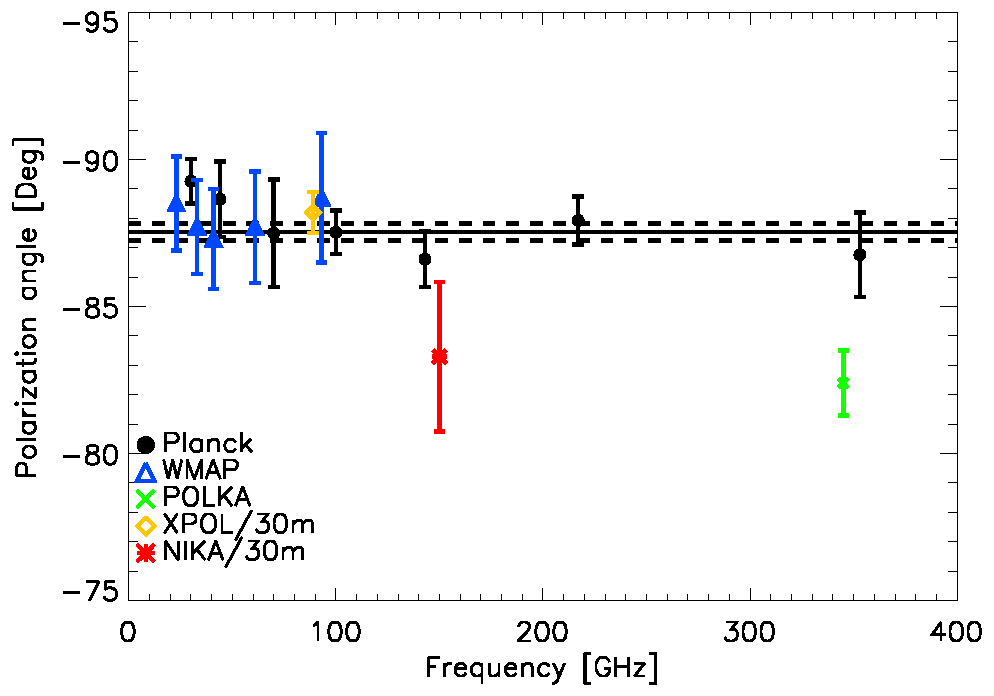
\includegraphics[width=1\linewidth,keepaspectratio]{figures/angle_comparison.pdf}} 
            \caption{{\it Top}: polarization degree as a function of frequency as measured by \Planck\ (black dots), WMAP (blue triangles), XPOL (green diamond) and \NIKA\ (red crosses). The \NIKA\ value has been estimated by integrating in a radius of $5^{\prime}$ as given by XPOL \citep{aumont2010}. The solid line represents the weighted-averaged degree of polarization accounting for low frequency values (\textless 200 GHz) and excluding XPOL.
            Dashed lines are the uncertainties.
            {\it Bottom}: polarization angles in Galactic coordinates for the same five experiments given above. The solid line represents the weighted-averaged polarization angles. Notice that the \NIKA\ value satisfies the condition I$_{pol}$ $>$ 3$\sigma_{I_{pol}}$ to avoid noise bias.} %accounting for all observations but SCUPOL and the dashed lines are the uncertainties.
%Notice that SCUPOL values \citep{scubapol} at 352 GHz have been estimated on maps covering only a region of 1.4$^\prime$ radius centered in the peak polarization intensity.}
\label{crab_p_angle_comparison}		
  \end{figure}

%\begin{table*}
 % \centering
  %    \begin{tabular}{ccccccccc}
  %    \hline
  %    \hline
  %     Experiments & Frequency & $\psi$ & $p$ & Comments \\ 
  %                                      & [GHz]  & [$^\circ$] & [\%] & \\
  %   \hline
  %   \hline
  %   \NIKA\ &  150 & -87.15 $\pm$ 0.01 (stat) $\pm$ 1.8 (syst) & 6.97$\pm$0.04 & This paper\\
  %  \Planck\ & 143 & -87.03 $\pm$ 0.97 & 7.19 $\pm$ 0.05 & \citep{2015arXiv150702058P} \\
  %   XPOL & 90 & -88.2 $\pm$ 0.7 & 8.8 $\pm$ 0.02 & \citep{aumont2010} \\
  %   \WMAP\ & 94 & -88.7 $\pm$ 2.2 & 7.13 $\pm$ 0.43 & \citep{2011ApJS..192...19W} \\
  %  \hline
  %  \hline   
  %  \end{tabular}
  %  \caption{Polarization angle and degree results obtained by four different experiments. For \NIKA\ and XPOL we estimate the values in five arcmin angular size, which corresponds to the beam of \Planck\ and \WMAP\ at 143 and 94 GHz, respectively.}
  %  \end{table*}


\section{Crab Spectral Energy Distribution in intensity and polarization}\label{sec:Polarization intensity Spectral Energy Density (SED)}
\subsection{Intensity}
The total intensity emission of the Crab nebula at radio and millimeter
wavelengths (from 1 to 500 GHz) is mainly due to synchrotron emission and can be
well described by a single power law of the form:
\begin{equation}
I_{\nu} = A(\nu / 1 {\bf GHz})^{\beta}
\end{equation}\label{eq:sync}
with spectral index $\beta$ = -0.296$\pm$0.06 \citep{baars1977absolute,macias2010}. Further, the Crab nebula is fading with time at a rate of $\alpha$ = 0.167$\pm$0.015 \% yr$^{-1}$ \citep{aller1985decrease}. 
These results suggest a low frequency emission produced by particles accelerated by the same magnetic field. \cite{macias2010} have shown also that there is no evidence for an extra synchrotron component and for a component of thermal dust emission at these frequencies. The direction of the polarization is therefore expected to be constant across the frequency range 30-300 GHz while the polarization degree may vary.

We show in Fig.~\ref{crab_SED} the flux of the Crab nebula as a function of frequency. The fluxes in the radio domain were taken from \cite{dmitrenko1970absolute} and \cite{1971IzVUZ..14..157V}. We also show microwave and mm wavelengths fluxes from \Archeops\ \citep{macias2007archeops}, \Planck\ \citep{2015arXiv150702058P}, WMAP \citep{2011ApJS..192...19W}, XPOL/30m \citep{aumont2010}, MAMBO/30m \citep{2002A&A...386.1044B} and GISMO/30m \citep{2011ApJ...734...54A}. The measured \NIKA\ total intensity flux at 150 GHz is shown in red.

\textbf{Accounting for the break shown by \Planck\ satellite data we assume a simple
two-power-law model\footnote{A detailed physical description of the SED of the
  Crab nebula is out of the scope of this paper.}:
\begin{equation}
I_{\nu} = \left\{ 
\begin{array}{rl}A_L(\nu/1GHz)^{\beta_L} &\mbox{$\nu<90$ GHz} \\
   A_H(\nu/1GHz)^{\beta_H} &\mbox{$\nu\geq90$ GHz}
  \end{array} \right.    
\end{equation}
By $\chi^2$-minimization we obtain the fit shown in cyan in Fig.~\ref{crab_SED},
where the cut-off frequency is 90 GHz and the knee frequencies are: 8 GHz and 100 GHz. 
The best-fit parameters obtained are:
$$\setlength\arraycolsep{0.1em}
 \begin{array}{rclcl}
  A_L&=& 507.7\pm0.1 ; \quad \quad   \beta_L = -0.3187\pm0.0001\\
  A_H&=& 216.4\pm0.3 ; \quad \beta_H = -0.7525\pm0.0003
 \end{array}
$$
We note that \NIKA\ data is consistent with this model at the 2$\sigma$ level. More data at mm wavelengths are needed to better understand the observed break of the SED around 90 GHz. }

\begin{figure}
  \centering
          { 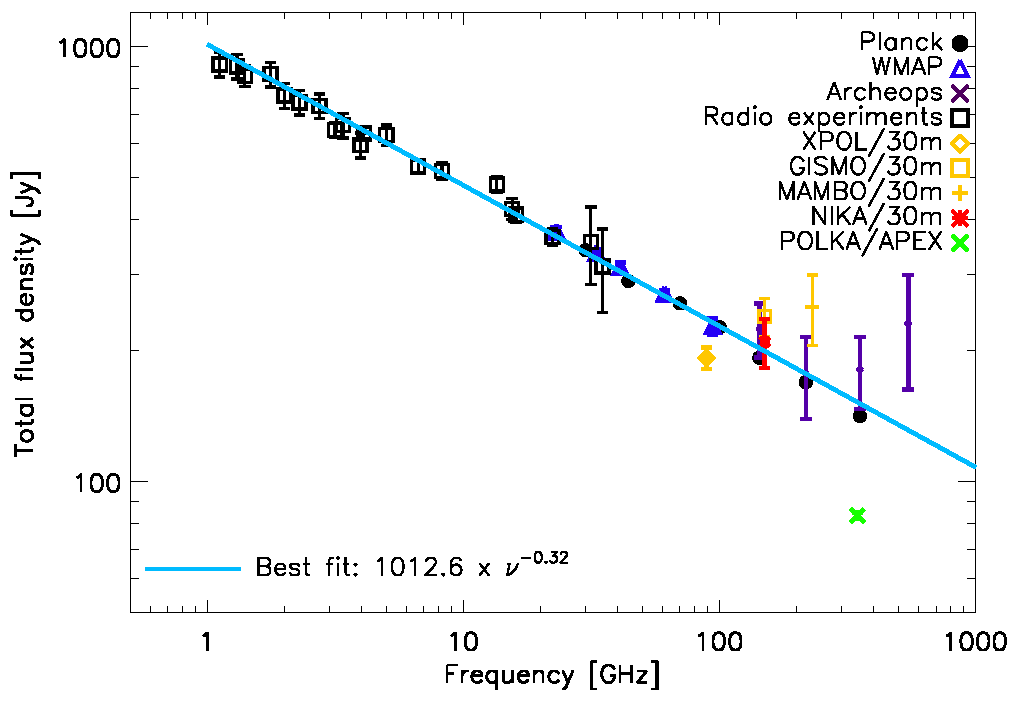
\includegraphics[width=1\linewidth,keepaspectratio]{figures/Crab_SED_int_test.pdf}}
           \caption{Crab nebula total intensity SED as obtained from \Planck\ \citep{2015arXiv150702058P}, \WMAP\ \citep{2011ApJS..192...19W}, Archeops \citep{macias2007archeops}, radio experiments \citep{dmitrenko1970absolute, 1971IzVUZ..14..157V}, XPOL/30m \citep{aumont2010}, \NIKA\/30m (this paper), MAMBO/30m \citep{2002A&A...386.1044B} and GISMO/30m \citep{2011ApJ...734...54A} data. The green line shows the model derived by a previous analysis discussed in \citep{macias2010}. The best-fit obtained by the analysis in this paper is shown in cyan line. Both, the best-fit models and the data account for the Crab nebula fading with the time.}
\label{crab_SED}		
  \end{figure} 

For illustration we also show in green line the best-fit model as result of a previous study \citet{macias2010}. 
Notice that in the plot both the best-fit modeland the data represented accounts for the fading of the source.
The estimated spectral index $\beta_L$ is slightly different if we compare with the previous estimation provided by \cite{macias2010}. This mainly concerns the addition of recently published results by \Planck\ \citep{2015arXiv150702058P} and  WMAP \citep{2011ApJS..192...19W}.
\NIKA\ camera agrees at 1 $\sigma$ level with both models. 
As already discussed above XPOL/30m total power emission is low with respect to expectations from both power law models.
 
The \Planck\ data at 100, 143, 217 and 353 GHz appears to be consistent with a much steeper SED with respect to the lower frequency data. This trend suggests  an extra emission component due to a different
population of relativistic electrons \citep{1965ARA&A...3..297G, 2012ApJ...760...96G} which to date has not been identified with other experiments. 

By contrast {\it Archeops}, MAMBO/30m, GISMO/30m
and \NIKA/30m do not seem to support such a low frequency break in the Crab nebula SED. In addition, \cite{macias2010} discusses this possibility but only for higher frequency above 1000~GHz, where few observations evidences a break in the power law. 

\textbf{This section figures out a clear inconsistency of recent \Planck\ data with low and high frequency data. In particular they show the evidence of a break in the power law around 90-100 GHz suggesting a different origin of the emission and/or the presence of a second population of electrons. This should be investigate more with high angular resolution observations which will permit to probe the small and large angular scales.}



\subsection{Polarization}
\textbf{Though the total power emission of the Crab nebula has been monitored over decades across a
large range of frequencies, the amount of polarization data is
very small.}
Recent results provided by
\Planck\ \citep{2015arXiv150702058P}, \WMAP\ \citep{2011ApJS..192...19W} and
XPOL \citep{aumont2010} together with \NIKA\ allow us to trace the spectral energy distribution of the polarized emission as shown in Fig.~\ref{crab_SED_ipol}.  

\textbf{\Planck\ data show an oscillating behaviour which is in contrast with what has been previously observed by \WMAP\ satellite.
The comparison between the two satellites at lower frequencies teases the question about the photometry of the \Planck\ LFI for different frequencies.
Whereas the \Planck\ data at 100 GHz shows again a break of the power law, the point at 353 GHz follows a completely different trend.
By contrast the \WMAP\ data, although only at low frequencies, show a self-consistent power law model.
Even if the comparison between the \WMAP\ and \Planck\ satellites is out the scope of this paper, we have decided to account for the two different trends shown by their results. Considering Eq.~\ref{eq:sync} as single power law like model for synchtron emission we use separately the \Planck\ and \WMAP\ data.}
In Fig.~\ref{crab_SED_ipol} the two best-fit models are shown in blanck and blue for \Planck\ and \WMAP\ data, respectively.
 
%This figure  show a tighter correlation of the XPOL measurement with other data because it is not affected by the Stokes $I$ quality.
%Furthermore, the average slope of the SED when approached by a single power-law seems to be different for the \Planck\ and \WMAP\ data.  To investigate this issue further we assume a power law model for the data as in Eq.~\ref{eq:sync}, and fit separately the \Planck\ and \WMAP\ data. We restrict the fit to the data with $\nu \textless$ 100 GHz. We show in Fig.~\ref{crab_SED_ipol} in black and blue the best-fit models for the \Planck\ and \WMAP\ data, respectively.

Accounting for fading the best-fit parameters A$_w$, $\beta_w$, A$_p$, $\beta_p$ for \WMAP\ and \Planck\ fits, respectively are:
%\begin{itemize}
%\item best-fit parameters for \WMAP\ only data:
%\begin{equation}
%A = 78.9\pm7.8 \quad , \quad \beta_p = -0.35\pm0.03;
%\end{equation}
%\item best-fit parameters for \Planck\ only data:
%\begin{equation}
%A = 179.1\pm15.4 \quad , \quad \beta_p = -0.54\pm0.02.
%\end{equation}
%\end{itemize}
$$
\setlength\arraycolsep{0.1em}
 \begin{array}{rclcl}
  A_w&=& 78.98\pm7.82 ; \quad \quad   \beta_w = -0.35\pm0.03\\
  A_p&=& 116.46\pm6.52 ; \quad \beta_p = -0.45\pm0.01
 \end{array}
$$

XPOL and \NIKA\ agree both power laws within 1$\sigma$ error bar. In this case the XPOL data are not affected by the Stokes $I$ map quality as in the case of the polarization degree measurement.
If the \WMAP\ best-fit model is in agreement with \Planck\ observations at 30, 100 and 353 GHz,  the \Planck\ best-fit model seems to overestimate the polarization flux at low frequency. In contrast
to the intensity data, here a 100 GHz break is less conspicuous.
We find no clear hint of a break in the polarization SED
at frequencies above 90 GHz, hence putting pressure on the hypothesis of multiple electron populations to explain the SED break in total power emission.

We have also estimated the spectral index of the Crab nebula polarization
emission at high frequency using the map obtained by SCUPOL \citep{scubapol} at 352 GHz (850
$\mu$m) and the \NIKA\ map. Considering only the region observed by SCUPOL we
obtain:
\begin{equation}
\beta_p = -0.33 \pm 0.01.
\end{equation}
This result is in good agreement with the \WMAP\ best-fit model spectral index.


\begin{figure}
  \centering
             { 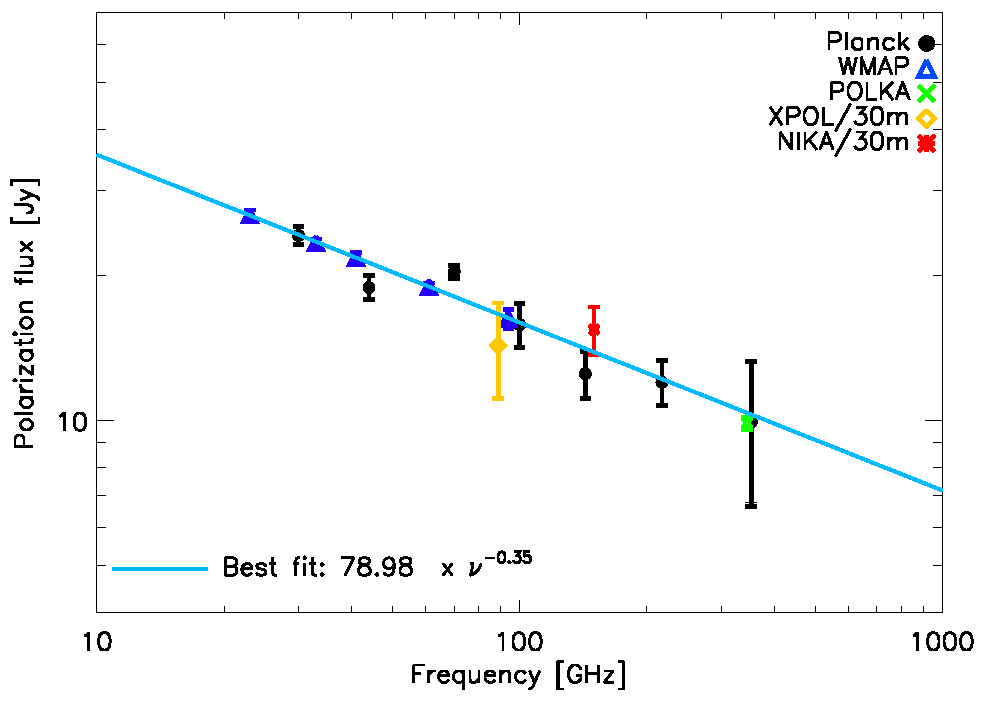
\includegraphics[width=1\linewidth,keepaspectratio]{figures/Crab_SED_ipol_test.pdf}}
           \caption{Crab nebula polarization flux SED as obtained from the \Planck\ \citep{2015arXiv150702058P}, \WMAP\ \citep{2011ApJS..192...19W} and \NIKA\ (this paper) data. The two best-fit models presented have been estimated using only WMAP data (blue line) or \Planck\ data only (black line).}
\label{crab_SED_ipol}		
  \end{figure} 
 \noindent
\textbf{From this analysis we noticed that the small amount of information at millimeter wavelengths in polarization emission is not conclusive but rather open several questions about the morphology of the polarized emission of the Crab nebula above 200 GHz. In the context of the \NIKA2\ instrument we aim to further investigate this aspect thanks to its polarized channel at 260 GHz.} 


\section{Conclusions}\label{sec:conclusions}
The Crab nebula is considered as a celestial standard calibrator for CMB experiments in
terms of polarization degree and angle. An absolute calibration is
particularly important for the measurement of the CMB polarization B-modes,
which are a window towards the physics of the early Universe.

We have reported in this paper first high angular resolution polarization observations
of the Crab nebula at 150 GHz with the \NIKA\ camera. These observations have
allowed us to accurately map the spatial distribution of the polarization
fraction and angle.  We find an averaged polarization angle of
-87.15$\pm$0.04$\pm$1.8 within a region of 5$^\prime$ radius with respect to the
central coordinates of the map R.A.: 05$^{h}$ 34$^{m}$ 31.09 s, Dec.:
+22$^{\circ}$ 00$^{\prime}$ 39.9$^{\prime\prime}$ (J2000).  This is consistent with
previous measurements from \Planck, \WMAP, and XPOL/30m.
Using all available polarization data to date we conclude that the
polarization angle of the Crab nebula is consistent with being constant with
frequency, from 23 GHz to 217 GHz, at arcmin scales with a value of
-88.1$^{\circ}$ $\pm$0.3 in Galactic coordinates.
In addition, there is a strong case for a constant polarization degree below 200 GHz. Above this frequency, \Planck\ results are not consistent to each other. 

Moreover, we have characterized the intensity and polarization SED of the Crab nebula. In intensity, recent \Planck\ data show a break in the SED that could be explained by the existence of different populations of relativistic electrons. However, they are inconsistent with other data. In polarization, we find that the data are overall consistent with a single power law spectrum as expected from synchrotron emission. However, we find some discrepancies between data sets, which will require further mm measurements at high resolution for a better understanding of the physics at play. Among future polarization experiments, \NIKAd\ \citep{calvo2016}, will provide high sensitive polarization observations of the Crab nebula adding a 260~GHz map at 11$^{\prime\prime}$ resolution.

\bibliography{bib_crab}

\vspace{0.2cm}
 \begin{acknowledgements}
We would like to thank the IRAM staff for their support during the \NIKA\ campaigns. 
The NIKA dilution cryostat has been designed and built at the Institut N\'eel. 
In particular, we acknowledge the crucial contribution of the Cryogenics Group, and 
in particular Gregory Garde, Henri Rodenas, Jean Paul Leggeri, Philippe Camus. 
This work has been partially funded by the Foundation Nanoscience Grenoble, the LabEx FOCUS ANR-11-LABX-0013 and 
the ANR under the contracts ``MKIDS'', ``NIKA'' and ANR-15-CE31-0017. 
This work has benefited from the support of the European Research Council Advanced Grant ORISTARS 
under the European Union's Seventh Framework Programme (Grant Agreement no. 291294).
We acknowledge fundings from the ENIGMASS French LabEx (R. A. and F. R.), 
the CNES post-doctoral fellowship program (R. A.),  the CNES doctoral fellowship program (A. R.) and 
the FOCUS French LabEx doctoral fellowship program (A. R.).
\end{acknowledgements}





\end{document}
